\documentclass{article}
\usepackage[a4paper,left=25mm,right=25mm,top=20mm,bottom=15mm]{geometry}
\usepackage[ngerman]{babel}   %   %Sprachunterstützung
\usepackage[utf8]{inputenc}   %Eingabecodierung
% \usepackage[T1]{fontenc}         %T1-Codierung Zeichensatz
\usepackage{amsmath}
\usepackage{amssymb}
\usepackage{amsfonts}

\usepackage{textcomp}
\usepackage{fancyhdr}
\usepackage{siunitx}
\usepackage{graphicx} 
\usepackage{minted} 


\usepackage{caption}
\newenvironment{code}{\captionsetup{type=listing}}{}
\usepackage[bookmarksopen=true]{hyperref}
\usepackage{float}
\usepackage{listings} % Für den Code

\usepackage[backend=bibtex,style=ieee]{biblatex}
\addbibresource{literatur.bib}

\usepackage{enumitem}
\usepackage{wasysym}
\usepackage{multicol} 
\usepackage{lmodern}
\usepackage{xcolor}
\usepackage{helvet}
\usepackage{tabularx}
\usepackage{pdfpages}
\usepackage{eurosym}
\usepackage[htt]{hyphenat}
\usepackage{circuitikz}
\usepackage{tikz}
\usepackage{longtable}
\usepackage{mdframed} % für Text Boxen

\usetikzlibrary{arrows,automata}
\usepackage{tikz-timing}
\usetikztiminglibrary[rising arrows]{clockarrows}
\usepackage{array,cellspace}
\usepackage{wrapfig}
\newcolumntype{L}[1]{>{\raggedright\arraybackslash}p{#1}} % linksbündig mit Breitenangabe
\newcolumntype{C}[1]{>{\centering\arraybackslash}p{#1}} % zentriert mit Breitenangabe
\newcolumntype{R}[1]{>{\raggedleft\arraybackslash}p{#1}} % rechtsbündig mit Breitenangabe
\newcolumntype{Y}{>{\centering\arraybackslash}X}
\newcolumntype{B}{>{\raggedright\arraybackslash}X}
\parskip=6pt
\setlength{\parindent}{0pt} 

\renewcommand{\arraystretch}{2.0}
\pagestyle{fancy}
\lfoot[\thepage]{SS 2024}
\rfoot[SS 2024]{\thepage}
\cfoot[]{ESP}

\rhead[]{\leftmark}
\lhead[\leftmark]{}

\usepackage{wrapfig}
% \renewcommand{\familydefault}{\sfdefault}

\begin{document}
\begin{titlepage}
\centering
    % \includegraphics[width=0.15\textwidth]{pic/thlogo/logo_TH-Koeln_CMYK_22pt.pdf}\par\vspace{1cm}

	{\Large I M A \par}
	{\huge\bfseries Intelligent Magic Audio\par}
	{Jonas Lux, Szymon Banasiak, Leon Braungardt\par}
	\vspace{2cm}
	{\Large\itshape Sommersemester 2024 \par}
	
	\vspace{6cm}
	\begin{figure}[h!]
		\centering
		\includegraphics[width=0.45\textwidth]{images/titelbild-xD.jpg}
		\label{fig:img-input-data-graph}
	\end{figure}
	\vfill
	
	
	
  
\end{titlepage}


\tableofcontents
\listoffigures
\newpage
%%%%%%%%%%%%%%%%%%%%%%%%%%%%%%%
\newpage
\section{Einleitung}
Bei dem Projekt ``Intelligent Magic Audio`` (IMA) handelt es sich um ein Projekt aus dem Modul ``Embedded Systems Praktikum`` (ESP) im Sommersemester 2024 an der TH Köln.

Ziel des Projekts ist die Entwicklung eines Audiosamplers im Eurorack-Standard, der auf einem STM32 Mikrocontroller basiert. Die Besonderheit des Samplers darin, dass auf eine SD-Karte geladenene Audiosamples über ein lokal laufendes Neuronales Netz (Edge AI) in fünf Klassen klassifiziert werden. Mit Hilfe von fünf Fadern und einer Suchfunktion kann der Nutzer sich passende Samples aus seiner Audiobibliothek vorschlagen und bei Bedarf wiedergeben lassen. 

Das Projektthema wurde aus Eigeninitiative vorgeschlagen, da es zentrale Aspekte der eingebetteten Systeme wie die Signal- bzw. Audioverarbeitung und den Umgang mit Peripheriegeräten vereint. Dies ermöglicht den Teammitgliedern, ihre Kenntnisse aus dem Modul ``Embedded Systems`` (ES) zu nutzen, um ein eigens entworfenes Produkt zu entwickeln und gleichzeitig ihre Fähigkeiten in ihren persönlichen Interessensgebieten zu vertiefen. Die Integration der Edge AI-Komponente bietet zudem die Möglichkeit, Erfahrungen im Betrieb neuronaler Netze auf Mikrocontrollern zu sammeln.

Der folgende Bericht bietet eine detaillierte Übersicht über den Projektverlauf, die verwendeten Technologien, die Herausforderungen und die Ergebnisse.

\newpage
\section{Detaillierte Projektbeschreibung}
\begin{itemize}
    \item Umriss des Projekts, ohne zu sehr auf Details wie Regler, Potis, exakte Display-Technologie usw. einzugehen. Dazu da, um dem Leser eine Idee zu geben, worum es geht und wie wir uns die Funktionalität vorgestellt haben.
    \item Bild von Faceplate
    \item Audiosampler für Eurorack Modularsystem (was ist das?)
    \item Problem: Schwierig die "richtigen" Samples zu finden $\Rightarrow$ Klassifizierung der Samples
    \item Suchfilter über Hardware-Interface (Regler)
    \item Anzeige der passenden Samples auf dem Display
    \item Auswählen/Abspielen mit Poti
    \item Eurorack Standard
\end{itemize}

	\subsection{Modulare Synthesizer}
	
	In der modernen elektronischen Musikproduktion erfreut sich die Modularität von Synthesizern wieder großer Beliebtheit. 
	Die Methoden, verschiedene Module von unterschiedlichen Herstellern miteinander zu kombinieren, erleben ein Revival. 
	Wo einst die Reise der elektronischen Musik begann, werden diese Ansätze erneut aufgegriffen.
	
	In den 1950er Jahren erzeugten die Pioniere der elektronischen Musik mit Labor- und Testequipment neue Klänge. 
	Signalgeneratoren, Filter und anderes technisches Gerät aus den Ingenieurlabors wurden funktional zu Musikinstrumenten umgewandelt – die elektronische Musik war geboren.
	
	In den 1990er Jahren, durch die bessere Zugänglichkeit und günstigeren Kosten von Chips und Halbleitern, fand dieses Mindset den Weg zu den Consumer-Musikproduzenten - Dieter Doepfer entwickelte den Eurorack-Standard für modulare Synthesizer. 
	Es werden 3,5 mm Stecker und Buchsen verwendet, um die verschiedenen Module miteinander zu "verpatchen". 
	Dabei werden ausschließlich Monokabel und Monosignale genutzt. Über diese Steckverbindungen werden alle Nutzsignale, die für die Produktion der Töne mit dem Synthesizer erforderlich sind, übertragen. 
	Audiosignale, Steuersignale und Triggersignale werden mit denselben Buchsen verbunden.
	
	Dies eröffnet enorme Möglichkeiten, die Klangpalette zu erweitern. So können beispielsweise Audiosignale zur Steuerung der Parameter eines Moduls verwendet werden, was kreative und innovative Patches ermöglicht.
	
	Auch technisch haben sich modulare Synthesizer weiterentwickelt. 
	Es wird vermehrt auf digitale Module gesetzt. 
	Die Zeit der Analog-Puristen ist vorbei; alle Möglichkeiten der digitalen Signalverarbeitung werden genutzt, um innovative Module zu entwerfen, die neue Methoden und Ideen in das eigene Rack bringen.
	
	Eine Unterkategorie der digitalen Module bilden die Audiosampler. Diese Module nehmen digitale Aufnahmen (Samples) von Klängen oder Musikstücken auf, speichern und spielen sie ab. Die Samples können durch verschiedene Trigger aktiviert und in unterschiedlichen Tonhöhen und Geschwindigkeiten abgespielt werden. 
	Audiosampler ermöglichen es Musikern, realistische Klänge von Instrumenten, Stimmen oder Umweltgeräuschen in ihre Musik zu integrieren und kreativ zu manipulieren.
	
	\newpage
	\subsection{Das Konzept}
	
	Es gibt durchaus Audiosampler mit ergonomischer Steuerung, großen hochauflösenden Displays und zahlreichen Knöpfen, um diese komplexen Audiomaschinen angenehm zu steuern. 
	Beispiele hierfür sind die legendäre MPC von AKAI oder der Octatrack von Elektron. 
	Diese Geräte sind jedoch aufgrund ihrer Bedienelemente und der damit einhergehenden Ergonomie so groß, dass sie unmöglich in ein Eurorack unterzubringen sind und oft unzählige Untermenüs besitzen.
	
	\begin{wrapfigure}{r}{0.4\textwidth} % Increase the width of the figure environment
		\vspace{-20pt + 0.02\textwidth}
		\hspace{0.02\textwidth} % Add horizontal space
		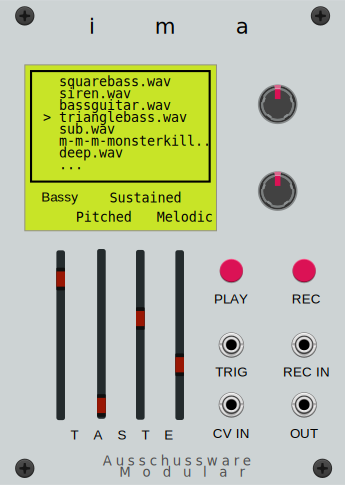
\includegraphics[width=0.38\textwidth]{pic/ima_mockup.png} % Keep the image size the same
		\caption{I M A Mockup Design}
		\vspace{-20pt}
	\end{wrapfigure}

	Daher sind Samplermodule im Eurorack-Standard häufig mit wenigen Features ausgestattet oder haben eine komplizierte, verschachtelte Bedienung. ``I M A`` (Intelligent Magic Audio) macht es Musikern hier deutlich einfacher! Der Schlüsselpunkt ist das gezielte Finden von Samples aus dem vorhandenen persistenten Speicher. Nur Samples des gewünschten Typs zu filtern, setzt normalerweise ein hohes Maß an manueller Sortierung und Ordnerstrukturierung voraus.
	
	
	Durch den neuronalgesteuerten Suchfilter von I M A kann eine Vorauswahl anhand musikalischer Parameter getroffen werden, ohne den kreativen Fluss des Künstlers zu unterbrechen.
	
	
	
	

\newpage
\section{Projektanforderungen}
\begin{itemize}
    \item Lastenheft: Welche Anforderungen gibt es? Falls nicht-funktionale Anforderungen existieren: in funktionale und nicht-funktionale unterteilen; LF nummeriert.
    \item (Pflichtenheft wird in Spezifikation integriert)
\end{itemize}
\newpage
\section{Spezifikation}
\subsection{Architektur}
\begin{itemize}
    \item Systemarchitektur: Gesamtdarstellung des Systems, wie Komponenten zusammenarbeiten
    \item Unterteilung in 3 Komponenten (Audio, User Interface, NN)
    \item Hier SA/RT Kontextdiagramm (evtl. ein Gesamt-Diagramm und pro Komponente ein weiteres)
    \item Hier SA/RT Modell für Zustandsautomat? und ggf. weitere Modelle
    
    \begin{figure}[H]
    	\centering
    	\includegraphics[width=0.8\textwidth]{images/04_spezifikation/kontextdiagramm_gesamt.drawio.png}
    	\caption{Kontextdiagramm des Gesamtsystems}
    	\label{fig:context_diagram_gesamt}
    \end{figure}
    
    %TODO: ausformulieren
    
    %TODO: Kontextdiagramme pro Untersystem
   
    
    \begin{figure}[H]
    	\centering
    	\includegraphics[width=1.0\textwidth]{images/04_spezifikation/fsm.drawio.png}
    	\caption{Zustandsautomat des Systems}
    	\label{fig:fsm}
    \end{figure}
    
    Folgendes Diagramm zeigt die Relation und Interaktion der 4 Komponenten miteinander.
    
    \begin{figure}[H]
    	\centering
    	\includegraphics[width=1.0\textwidth]{images/04_spezifikation/komponentendiagramm.drawio.png}
    	\caption{Komponentendiagramm}
    	\label{fig:komponentendiagramm}
    \end{figure}
\end{itemize}
\newpage
\subsection{Technische Spezifikation}
\begin{itemize}
    \item Welche Hardware wird für welchen LF und warum benötigt?
    \item Warum dieser Standard/Protokoll?
    \item Eurorack Standard
\end{itemize}


\subsubsection{Hardware}

\textcolor{red}{TODO: Hardware eklärung und Pin belegung trennen}

\textcolor{red}{TODO: PIN Belegung an mein Projekt anpassen}

\textcolor{red}{TODO: Überarbeitung der Hardware Erklärung mehr Technisch}

\textcolor{red}{TODO: Pinbelegung in einer eigene Tabelle(Mit Pull Up, Pull Down etc.)}

\textbf{Komponenten/LF1/:} \\


\textbf{(Encoder)} \\

\textbf{Elektorisch} 3.3V

\textbf{Mechanisch} GPIO Pins \textcolor{red}{PD1 PD0 PG1}
\\

Zur Auswahl der Samples und zum Navigieren durch das Menü benötigen wir einen Rotary-Encoder mit einem Switch Button.Das Empfangen der A und B Signale des Encoders erfolgt über die Pins PD0 und PD1. Der Encoder ist so konfiguriert das wen PD0 und PD1 auf high sind der Encoder den Cursor incrementiert. Wen PD0 high und PD1 low ist wird der Cursor runtergezählt.
Das Drücken des Switch über den Pin PG1. Durch das drücken des Switch-Buttons wird der Pin PG1 auf high gesetzt und die Auswahl des Samples wird übernommen.

\begin{itemize}
	\item \textbf{Präzise Steuerung:} Der Encoder ermöglicht eine präzise Steuerung des Cursors auf dem Display.
	
	\item \textbf{Benutzerfreundlichkeit:} Der Benutzer kann durch die Liste navigieren und ein Sample auswählen. Die Kombination aus Drehbewegung und Druckknopf-Funktionalität macht den Encoder intuitiv.  
\end{itemize}





\textbf{(LCD-Display)} \\

\textbf{Elektorisch} 5.0V

\textbf{Mechanisch} GPIO Pins  \textcolor{red}{PF0 PF1} \\

Zur Visualiesierung der Sampels haben wir einen Monochronen LCD-Display benutzt. Im zusammenspiel mit dem Encoder ermöglicht es eine gute Navigation durch den gewünschten Samplepool. Die Daten werden über den Output Pin  \textcolor{red}{PF0} an den SDA des Displays übertragen. Der Takt wird über den Pin  \textcolor{red}{PF1} an den SCL übertragen. Das Display wird mit 20 FPS betrieben und mit hilfe von \textcolor{red}{Timer tim5} geupdated.

\begin{itemize}
	\item \textbf{Klare Visualisierung:} LCD-Displays bieten eine klare und gut lesbare Darstellung von Text und Grafiken.
	
	\item \textbf{Energieeffizienz:} LCDs sind energieeffizient.
	
	\item \textbf{Verfügbarkeit:} LCD-Displays sind weit verbreitet und leicht zu beschaffen, was die Beschaffungskosten senkt und die Integration erleichtert.
	
	\item \textbf{Anpassbarkeit:} Sie können einfach an verschiedene Layouts und Designs angepasst werden.
\end{itemize}


Die Kombination aus Encoder und LCD-Display bietet somit eine effiziente und benutzerfreundliche Lösung für die Steuerung und Anzeige in einem Audio Sample Recorder und Playback Device.

\newpage
\textbf{Komponenten/LF2/:}\\

\textbf{(Schiebe-Potentiometer)}\\

\textbf{Elektorisch} 3.3V

\textbf{Mechanisch} GPIO Pins  \textcolor{red}{PA0 PA3 PA4 PC0 PC3} \\

Für die Filterfunktion benötigen wir 5 Potentiometer. Es wird zyklisch die Ausgangsspannung des Schleifers abgegriffen die die Teilspannung zwichen den VCC und dem GND darstellt. Dies erfolgt mit Hilfe vom ADC und dem DMA. Die Auswertung der Spannung erfolgt über die Pins  \textcolor{red}{PA0 PA3 PA4 PC0 PC3}. Die Pins  \textcolor{red}{PA0 PA3 PA4 PC0} sind für die Klassen zuständig  \textcolor{red}{PC3} für den Schwellenwert an erlaubter abweichung.

\begin{itemize}
	\item \textbf{Präzise Steuerung und feine Abstimmung:} Ein Potentiometer ermöglicht eine stufenlose und präzise Einstellung. Durch das Schieben des Potentiometers kann der Benutzer den Cursor in kleinen, genauen Schritten bewegen.
	\item \textbf{Einfache Bedienung und intuitive Nutzung:} Potentiometer sind einfach und intuitiv zu bedienen.
	\item \textbf{Robuste Mechanik und Zuverlässigkeit:} Potentiometer sind mechanisch robust und zuverlässig. Sie können eine hohe Anzahl von Schiebezyklen ohne an Genauigkeit oder Funktionalität zu verlieren.
	\item \textbf{Direkte visuelle Rückmeldung:} Durch die sofortige visuelle Rückmeldung auf dem LCD-Display kann der Benutzer sofort sehen, wie sich die Bewegung des Potentiometers auf die Position des Cursors auswirkt.
\end{itemize}

\textbf{(ADC)}\\

\textbf{ADC} (Analog Digital Converter) wird benutzt, um die Ausgangsspannung an den Schleifern zu digitalisieren und in Zahlen zu fassen. Dies erfolgt über die Pins \textcolor{red}{PA0, PA3, PA4, PC0, PC3}, die als Schnittstellen parallel der Reihenfolge der Channels \textcolor{red}{0, 2, 3, 10, 13} dienen. Jedes Mal, wenn an der Ausgangsspannung eines der Schleifer eine Veränderung wahrgenommen wird, startet eine Interrupt Service Routine, die auf einer Callback-Methode basiert. Diese berechnet dann einen geglätteten Endwert für die Ausgangsspannung. \\

\textbf{(DMA)}\\

\textbf{DMA} (Direct Memory Access) wird gestartet, um die Werte, die an den Pins des ADC liegen, zyklisch zu pollen. Er wird zeitbasiert mit einem \textcolor{red}{Timer tim5} gestartet und in der Callback nach der Glättung der kumulierten ADC-Werte gestoppt.

\textbf{\textcolor{red}{Timer:}} Timer5, Internal Clock, One Pulse Mode \\
\textbf{\textcolor{red}{Data Width:}} Word Übertragung von 32-Bit-Datenblöcken \\
\textbf{\textcolor{red}{Mode:}} Circular \\

\textbf{(LCD-Display)}\\

Der LCD-Display ist der gleiche wie im \textcolor{red}{/LF01/} beschrieben. Dieser dient zur Darstellung der Fader Einstellung in prozentualer Form.

\newpage

\subsubsection{Pinout}
\begin{longtable}[c]{|p{2.5cm}|p{1cm}|p{2.5cm}|p{2.5cm}|p{2.5cm}|p{3cm}|}
	\hline
	\textbf{Komponente} & \textbf{PIN} & \textbf{Signal-On-PIN} &  \textbf{GPIO-Mode} & \textbf{GPIO-Pull-Up/Pull-Down } & \textbf{User-Label}\\
	\hline
	Encoder Menü & PA0 & n/a & EIMRETD & PULL UP & enc\_a\_clk\_in1 \\
	\hline
	& PA1 & n/a &  INPUT & PULL UP & enc\_a\_dt\_in2 \\
	\hline
	& PA4 & n/a & EIMRETD & PULL UP & enc\_a\_switch\_in3 \\
	\hline
	ADC & PA6 & ADC1\_IN6 & ANALOG & NPU NPD & FADER1 \\
	\hline
	& PA7 & ADC1\_IN7 & ANALOG & NPU NPD & FADER2 \\
	\hline
	& PB0 & ADC1\_IN8 & ANALOG & NPU NPD & FADER3 \\
	\hline
	& PB1 & ADC1\_IN9 & ANALOG & NPU NPD & FADER4 \\
	\hline
	& PC0 & ADC1\_IN10 & ANALOG & NPU NPD & FADER5 \\	
	\hline
	I2C & PB6 &I2C1\_SCL & AFOD & PULL UP & n/a \\
	\hline
	& PB7 &I2C1\_SDA & AFOD & PULL UP & n/a \\
	\hline
	SDIO & PC8 & SDIO\_D0 & AFPP & PULL UP & n/a \\
	\hline
	& PC9 & SDIO\_D1 & AFPP & PULL UP & n/a \\
	\hline
	& PC10 & SDIO\_D2 & AFPP & PULL UP & n/a \\
	\hline
	& PC11 & SDIO\_D3 & AFPP & PULL UP & n/a \\
	\hline
	& PC12 & SDIO\_CK & AFPP & NPU NPD & n/a \\
	\hline
	& PD2 & SDIO\_CMD & AFPP & PULL UP & n/a \\
	\hline
	I2S & PB10 & IS2\_CK & AFPP  & NPU NPD & n/a \\
	\hline
	& PB12 & IS2\_WS & AFPP & NPU NPD & n/a \\
	\hline
	& PC3 & IS2\_SD & AFPP & NPU NPD &  n/a \\
	\hline
	& PC6 & IS2\_MCK & AFPP & NPU NPD &  n/a \\
	\hline
\end{longtable}

\newpage

\subsection{Schnittstellenbeschreibung und Integration der Komponenten}
\begin{itemize}
    \item Planung der Schnittstellen zwischen den Komponenten
    \item Einfaches Diagramm in DrawIO:
    \begin{itemize}
        \item Zwischen Jonas und Leon: \texttt{downsampleandread1024()}
        \item Zwischen Syzmon und Jonas: \texttt{filemanager struct}, etc.
        \item Zwischen Szymon und Leon: \texttt{filemanager struct}
    \end{itemize}
    
    
    Folgendes Diagramm zeigt die Relation und Interaktion der 4 Komponenten miteinander.
    
    \begin{figure}[H]
    	\centering
    	\includegraphics[width=1.0\textwidth]{images/04_spezifikation/komponentendiagramm.drawio.png}
    	\caption{Komponentendiagramm}
    	\label{fig:komponentendiagramm}
    \end{figure}
    
\end{itemize}
\newpage
\section{Durchführung}
Im Anschluss an die Spezifikation des Systems folgt die Beschreibung der Umsetzung der einzelnen Komponenten. In diesem Abschnitt werden die angewandten Ansätze und Methodiken erörtert, die zur Realisierung der einzelnen Komponenten genutzt wurden. Weiterhin wird die Herangehensweise beschrieben, sowie wichtige Erkenntnisse und aufgetretene Probleme während der Implementierungsphase dokumentiert. Abschließend wird die Thematik der Gesamtintegration behandelt, einschließlich der Herausforderungen und der Gründe, warum eine vollständige Integration nicht erreicht wurde.

\subsection{Audio Engine des Samplers}

Die Hauptfunktionalität eines Audiosamplers ist natürlich das Aufnehmen und Abspielen von Audiosamples. 

Der ausgesuchte PCM5102a Audio Codec verfügt lediglich über einen Ausgabestream, was eine Neubestellung eines Codecs mit In- und Output Stream erfordern würde.

Angesichts des ohnehin schon ambitionierten Featureumfangs und der damit verbundenen Zeitknappheit, wurde die Aufnahmefunktion \textbf{\hyperlink{lf-audiorecord}{LF04}} gestrichen, sodass der Prototyp zu einer reinen ``Sample-Playback`` Maschine wird. 

Das folgende Kapitel befasst sich mit der Implementierung und Ansteuerung der Audiowiedergabe über den Audio Codec und aller verbundenen DSP-Operationen.

Zunächst folgt eine Erläuterung des grundlegenden Signalfluss der Audioengine:

\subsubsection{Signalfluss der Audioengine}

Alle Audiosamples werden auf einer angeschlossen \textbf{SD Karte} persistent gespeichert. Diese werden dann immer stückweise mit dem \textbf{FATFS} Dateisystem, welches für eingebettete Systeme optimiert ist, in die Applikationslogik und somit den Audiopufferspeicher geladen. 

Von hier aus reicht die \textbf{DMA} den Buffer per \textbf{I2S} Protokoll an den \textbf{Audio Codec} weiter. 

Der Audio Codec wandelt die digitalen PCM Signale in eine analoges Signal mit Line-Level. %(TODO: Line Pegel elektrisch angeben). evtl auf Datenblatt verweisen?

\begin{figure}[h!]
	\centering
	\includegraphics[width=0.9\textwidth]{images/08_durchfuehrung/audio/audio_signalflow.drawio.png}
	\caption{Digitaler Audio Signalfluss}
	\label{fig:audio_signalflow}
\end{figure}


\subsubsection{Latenzen}

Echtzeitfähigkeit ist ein kritischer Aspekt bei elektronischen Audioinstrumenten. 
Eine niedrige Latenz ist entscheidend, um rhythmisch präzise und ``tight`` zu spielen, besonders wenn mehrere Instrumente miteinander synchronisiert werden müssen.

Die maximale Latenz, die ein menschlicher Profimusiker noch akzeptieren kann, liegt bei etwa 20ms. Diese Richtwert basiert auf der Wahrnehmungsgrenze, bei der Musiker und Live-Performern keine signifikante zeitliche Verzögerung zwischen dem Triggern eines Samples und dessen tatsächlichem Output am Ausgang spüren. \cite{latency-experiment}

Um die Latenz auf ein Minimum zu reduzieren und sicherzustellen, dass elektronische Audioinstrumente reaktionsschnell und synchronisiert sind, können folgende Methoden angewendet werden:

\paragraph{Dimensionierung der Buffersize}\

Die erste Einstellungsmöglichkeit ist die \textit{Buffersize}.
Das ist die Größe (in Bytes) des Audiobuffers.
Je kleiner der Audiobuffer, desto öfter pro Sekunde gibt die DMA dessen Inhalt an den Audio Codec weiter.

Das bringt jedoch auch Performanceeinbußen mit sich: Bei kleinen Audiobuffern hat die CPU, je nach Komplexität der durchzuführenden DSP-Operationen, möglicherweise nicht genug Zeit, um den gesamten Buffer zu verarbeiten.
Ein nur teils verarbeiteter Buffer kann hörbare Knackser und Störgeräusche am Ausgangssignal verursachen.

Hier gilt es also, die kleinstmögliche Buffersize zu ermitteln, ohne dass Störgeräusche auftreten.
Nach Experimentieren hat sich ein Wert von \textbf{128 Bytes} als adäquat herausgestellt.

\paragraph{Verwendung von Double Buffering}\

Double Buffering ermöglicht es, Daten in einem Pufferspeicher zu verarbeiten, während gleichzeitig ein anderer Puffer für die Eingabe oder Ausgabe verwendet wird. Dies reduziert Verzögerungen und ermöglicht eine nahtlose Datenverarbeitung, da der Prozessor nicht auf das Ende einer Übertragung oder Berechnung warten muss, bevor er fortfahren kann. \cite{double-buffering}

\begin{figure}[H]
	\centering
	\includegraphics[width=0.6\textwidth]{images/08_durchfuehrung/audio/double_buffering.drawio.png}
	\caption{Double Buffering mit DMA und DSP}
	\label{fig:double_buffering}
\end{figure}


Bei I M A wird wird der Audiobuffer halbiert. %TODO: besser formulieren
Durch den Pointer \mintinline{c}|int16_t *outBufPtr| wird mit der DSP die Hälfte bearbeitet, die gerade nicht von der DMA übertragen wird.

In den Callback-Funktionen \mintinline{c}|HAL_I2S_TxHalfCpltCallback()| und \mintinline{c}|HAL_I2S_TxCpltCallback()| wird der Pointer auf die jeweilige Hälfte des Buffers, also auf (wie in  \textbf{\autoref{fig:double_buffering}} beschrieben:
\textbf{Buffer~A} und \textbf{Buffer~B}) gesetzt.


\inputminted[firstline=28, lastline=31]{c}{../../f401_sd_card_audio_codec_test/Core/Src/audio.c}

\inputminted[firstline=40, lastline=43]{c}{../../f401_sd_card_audio_codec_test/Core/Src/audio.c}


Diese Callbacks, werden systembedingt aufgerufen, sobald die DMA die erste Hälfte oder den gesamten Buffer übertragen hat. Sie eignen sich daher sehr gut um den Pointer zu setzen.

"Sobald das Flag \mintinline{c}|dma_dataReady == true| gesetzt ist, wird die nächste Bufferhälfte von der SD-Karte gelesen."

\paragraph{Latenzmessung}

Die Latenzmessung im Abschnitt \ref{test-latenzmessung} zeigt, dass die gemessene Latenz von Trigger Input bis Audioausgang mit \SI{6.7}{\milli\second} sehr zufriedenstellend ist, was ein erfolgreiches Zusammenspiel mit anderen elektronischen Instrumenten ermöglicht.


\subsubsection{PCM5102a und I2S}

Ein sehr weit verbreitetes Protokoll zur digitalen Audioübertragung ist I2S. Viele Codecs, so auch der PCM5102a, unterstützen dieses Protokoll.

I2S (Inter-IC Sound) ist ein Standard für die digitale Übertragung von Audiodaten zwischen integrierten Schaltkreisen (ICs). Es wurde entwickelt, um die Kommunikation von digitalen Audiodaten zwischen verschiedenen Komponenten wie Mikrofonen, DACs (Digital-Analog-Wandler) und ADCs (Analog-Digital-Wandler) zu ermöglichen. \cite{i2s-reference}

Der PCM5102a erkennt komfortablerweise die eingehende Samplerate anhand der Bitclock.
Anders als bei vielen Audio Codecs ist keine zusätzliche Konfiguration des Chips über ein Kommunikationsprotokoll, wie I2C notwending.

Somit fallen auch keine Treiber für diesen Chip an, was die Einbindung sehr vereinfacht.

Die I2S Signale des PCM5102a sind:

\begin{itemize}
	\item \textbf{SCK (System Clock)}: Dieser Takt wird für den Betrieb des internen Digitalfilters und des DAC-Kerns verwendet. Er kann entweder extern bereitgestellt oder intern vom PCM5102a erzeugt werden.
	\item \textbf{BCK (Bit Clock)}: Dieser Takt signalisiert den Beginn jedes Bits im Datenwort. Der BCK wird verwendet, um die Daten auf der Datenleitung (DIN) zu takten.
	\item \textbf{LCK (Left/Right Clock)}: Auch als Word Select oder Frame Sync bekannt. Dieser Takt signalisiert den Beginn eines neuen Audioframes und zeigt an, ob die aktuellen Daten den linken oder rechten Kanal darstellen.
	\item \textbf{DIN (Digital Input)}: Dies ist die Datenleitung, über die die PCM-Audiodaten übertragen werden.
\end{itemize}

Der Einfachheit halber wird eine festgelegte Samplerate und nur Stereo-Samples verwendet.

\subsubsection{SD Karte}

Durch den sehr begrenzter RAM-Speicher des NUCLEO F401re Boards , ist es notwendig die Daten in Echtzeit von der SD-Karte zu streamen. Das setzt bei Stereo PCM Dateien, mit den gängigen Parametern, eine bestimmte Datenrate \( R \) voraus:

\begin{itemize}
	\item Abtastrate (Sampling Rate): 44.100 Hz (44,1 kHz)
	\item Bit-Tiefe: 16 Bit
	\item Kanäle: 2 (Stereo)
\end{itemize}


Die Datenrate \( R \) berechnet sich aus:

\[
R = \text{Sampling Rate} \times \text{Bit-Tiefe} \times \text{Anzahl der Kanäle}
\]



\[
R = 44{,}100 \, \text{Hz} \times 16 \, \text{bit} \times 2
\]

\[
R = 1{,}411{,}200 \, \text{bit/s} \approx 0.168 \, \text{MB/s}
\]


Theoretisch hätte eine Implementierung des FATFS-Dateisystems über SPI ausreichen müssen, um diese Datenraten zu bewältigen. 

Um die SDIO-Schnittstelle in das FATFS-Dateisystem zu integrieren, mussten zunächst Treiber entwickelt werden. Diese Treiber mappen die üblichen Dateioperationen wie \mintinline{c}|f_open()|, \mintinline{c}|f_read()| usw. über die SPI-Schnittstelle.


In der Praxis stellte sich jedoch heraus, dass der Audiobuffer nicht schnell genug gefüllt worden ist, was starke Knackser und Störgeräusche mit sich gebracht hat.

\begin{wrapfigure}{r}{0.3\textwidth} % Increase the width of the figure environment
	\vspace{-20pt}
	\fbox{\includegraphics[width=0.3\textwidth]{images/08_durchfuehrung/audio/cubemx_sdio.png}}
	\caption{CubeMX FATFS SDIO Einbindung}
	\label{fig:cubemx_sdio}
\end{wrapfigure}

Dies erwies sich als äußerst vorteilhaft, da die SDIO-Implementierung zusammen mit FATFS direkt im Konfigurationstool von STM, \textbf{CubeMX}, ausgewählt werden kann. Die benötigten Treiber werden von CubeMX automatisch generiert und integrieren sich problemlos in das Dateisystem.

\subsubsection{Playback und Pitched Playback}

Der Audioplayer unterstützt das Abspielen von WAV-Dateien mit Tonhöhenanpassung. Dies wird durch die Verwendung von DMA zur Übertragung über I2S erreicht. Die Audiowiedergabe erfolgt mit dynamischer Anpassung der Abspielgeschwindigkeit, was eine Echtzeit-Tonhöhenänderung ermöglicht.

Die Funktion \mintinline{c}|wavPlayPitched(WavPlayer *player)| liest Audiodaten von der SD-Karte:

\mint{c}|bytesRead = fillHalfBufferFromSD(player, true);|

wobei die Funktion \mintinline{c}|fillHalfBufferFromSD()|, die Anzahl der benötigten Samples für den Buffer, dynamisch anhand der Abspielgeschwindigkeit errechnet.

\paragraph{Pitchfaktor}

Ein Pitchfaktor größer als 1.0 bedeutet, dass die Wiedergabegeschwindigkeit erhöht wird. Um diese höhere Geschwindigkeit zu kompensieren, müssen mehr Samples in den Puffer geladen werden. Das liegt daran, dass mehr Daten pro Zeiteinheit benötigt werden, um die schnellere Wiedergabe zu unterstützen.

Ein Pitchfaktor kleiner als 1.0 reduziert die Wiedergabegeschwindigkeit. In diesem Fall werden weniger Samples benötigt, weil sich die Daten im Puffer wiederholen. Das bedeutet, dass der Puffer nicht so schnell gefüllt werden muss, da die Audio-Daten langsamer abgespielt werden.

\paragraph{PCM-Stereocodierung}

Beim Füllen des Audiobuffers mit einem Pitchfaktor \( \neq 0 \) muss darauf geachtet werden, dass die PCM Stereo-Codierung korrekt beachtet wird. 
Im PCM Stereo-Format repräsentieren alle geraden Samples im Buffer den linken Kanal, während die ungeraden Samples den rechten Kanal darstellen.

Wenn der Pitchfaktor verändert wird, können Samples entweder übersprungen oder doppelt abgespielt werden. Dabei ist es entscheidend, dass die richtigen Samples für den linken und rechten Kanal ausgewählt werden. Der folgende Code sorgt dafür, dass diese Auswahl korrekt erfolgt:

\begin{minted}{c}
	leftReadIndex = (leftReadIndex + 1) & ~1;
	rightReadIndex = leftReadIndex + 1;
\end{minted}


\noindent
Hier ist eine detaillierte Erklärung dieser Operationen:

\begin{enumerate}
	\item \textbf{Sicherstellung eines geraden Indexes:} \\
	Der Code:
	\begin{quote}
		\mintinline{c}|leftReadIndex = (leftReadIndex + 1) & ~1;|
	\end{quote}
	sorgt dafür, dass \mintinline{c}|leftReadIndex| immer eine gerade Zahl ist. Zunächst wird \mintinline{c}|1| zu \mintinline{c}|leftReadIndex| addiert, um eine gerade Zahl zu erhalten. 
	
	Die bitweise UND-Operation mit \mintinline{c}|~1| (der negierten Zahl 1) entfernt das niedrigstwertige Bit von \mintinline{c}|leftReadIndex + 1|, wodurch der Wert zu einer geraden Zahl wird. 
	
	Zum Beispiel wird aus 5 (ungerade) 6 (gerade), und aus 7 (ungerade) wird ebenfalls 6 (gerade).
	
	\item \textbf{Berechnung des \mintinline{c}|rightReadIndex|:} \\
	Der Index für das rechte Sample wird durch die folgende Zeile berechnet:
	\begin{quote}
		\mintinline{c}|rightReadIndex = leftReadIndex + 1;|
	\end{quote}
	Nachdem \mintinline{c}|leftReadIndex| als gerade Zahl festgelegt wurde, ist \mintinline{c}|rightReadIndex| automatisch der nächste Index, der ungerade ist. Dies entspricht dem Format von PCM Stereo-Samples, bei dem gerade Indizes für den linken Kanal und ungerade Indizes für den rechten Kanal verwendet werden.
\end{enumerate}

Diese Schritte stellen sicher, dass die berechneten Indizes korrekt auf die im Stereo-PCM-Format erwarteten Positionen verweisen, indem sie sicherstellen, dass der Puffer die richtigen Daten für den linken und rechten Kanal enthält.


\subsubsection{Downsampling eines Audiochunks für die Verarbeitung von Audio durch das Neuronalen Netzes}
\label{sec:audio-downsampling}


Damit die proprietäre ``STM32\_AI\_AudioPreprocessing\_Library`` (Abschnitt \ref{stm32-cube-ai}) die Audiodaten in Spektrogramme umwandeln kann, müssen die Daten zunächst ins korrekte Format gebracht werden. Für die Umwandlung erwartet die Library \SI{16}{\kilo\hertz} Samplerate, Mono Dateien.

In der Datei
\path{/f401_sd_card_audio_codec_test/Core/Src/audioPreprocessor.c}
finden sich alle Funktionen, die das Audiopreprocessing der Audiodatei für die Klassifizierung betreffen.

Die Funktion 
\mint{c}|uint32_t downsample_to_1024_samples(FIL *file, int16_t outChunk[NUM_SAMPLES_CHUNK_OUT])|
liest einen Audiochunk aus einer Datei von der SD Karte, konvertiert die Stereo-Samples in Mono und führt anschließend eine Abtastratenreduktion (Downsampling) durch. Die verarbeiteten Samples werden im \mintinline{c}|outChunk|-Buffer gespeichert. Die Funktion arbeitet blockweise und gibt die Anzahl der heruntergesampelten Samples zurück. 

Zunächst werden die Eingabedaten in den Puffer \mintinline{c}|inputChunk| eingelesen. Die Stereo-Samples werden durch Mittelung der linken und rechten Kanäle in Mono umgewandelt und in den Puffer \mintinline{c}|currentInBlockMono| geschrieben. Anschließend wird die Funktion \mintinline{c}|downsample_Block| aufgerufen, die die eigentliche Abtastratenreduktion und FIR-Filterung durchführt.

Die Funktion \mintinline{c}|downsample_Block| konvertiert die 16-Bit-Integer-Audiodaten in ein Fließkommaformat, führt FIR-Filterung und Dezimierung durch und konvertiert die gefilterten Samples zurück in das 16-Bit-Integer-Format. Die verarbeiteten Daten werden dann in den Zielpuffer geschrieben.

Um Aliasing beim heruntergesampleten Audiomaterial zu vermeiden, werden die benötigten Samples vor dem Downsampling mit einem FIR Highcut geglättet. 
Die Koeffizienten können mit Filterdesign-Softwares, wie \url{http://t-filter.engineerjs.com} generiert werden. Es wurde ein Filter mit 57 Koeffizienten gewählt, der eine gute Balance zwischen Performance und Ripple bietet. 
Wie in Abbildung \ref{fig:fir-filter} zu sehen, bietet der Filter ab \SI{16}{\kilo\hertz} eine recht steile Flanke bis \SI{-45}{\deci\bel} Abschwächung.

\begin{figure}[h!]
	\centering
	\includegraphics[width=0.7\textwidth]{images/08_durchfuehrung/audio/fir_lowpass.png}
	\caption{Anti-Aliasing FIR Lowpass Filter}
	\label{fig:fir-filter}
\end{figure}

Die Open Source CMSIS DSP Library (Link) bietet direkt eine optimierte Funktion, welche die FIR-Filterung, sowie das eigentliche Downsampling kombiniert: \mintinline{c}|arm_fir_decimate_f32|.



\subsection{Klassifizierung von Audiodateien durch ein Neuronales Netz}
Durch das neuronale Netz sollen digitale Audiodateien (Audiosamples) mit variabler Länge in fünf Merkmalsklassen klassifiziert werden. Dabei kann ein Datenpunkt, also ein Audiosample, mehreren Merkmalsklassen zugehörig sein. Dies wird als ``Multi-Label-Klassifizierung`` bezeichnet \cite{multilabel-classification}. Wird eine Audiodatei (Eingabevektor) zur Klassifizierung in das neuronale Netz eingegeben, erhält man als Ausgabe einen Ausgabevektor von fünf Werten zwischen 0.00 und 1.00, wobei jeder der fünf Werte  die Ähnlichkeit mit einer der fünf Merkmalsklassen repräsentiert (0.00 $\equiv$ keine Ähnlichkeit, 1.00 $\equiv$ Übereinstimmung). Die Merkmalsklassen werden wie folgt definiert:
    \begin{itemize}
        \item \textbf{bass:} Das Audiosample enthält Töne aus dem tiefen Frequenzspektrum
       	\item \textbf{pitched:} Das Audiosample enthält Töne aus dem hohen Frequenzspektrum
        \item \textbf{melodic:} Das Audiosample enthält melodische Elemente
        \item \textbf{rhythmic:} Das Audiosample enthält rhytmische Elemente
        \item \textbf{sustained:} Das Audiosample enthält ``flächige`` Elemente, also ``langgezogene`` Töne
    \end{itemize}

Dieses neuronale Netz wird mit selbst generierten Trainingsdaten trainiert und anschließend als fertiges Modell mittels dem STM32 proprietären Tool ``STM32Cube.AI`` in C-Code umgewandelt. Damit kann das Neuronale Netz im eigenen Code als normale C-Funktion verwendet werden, mit dem Eingabevektor (Audiodaten) als Funktionsparameter und dem Ausgabevektor (Klassifikationsergebnis) als Rückgabewert. \cite{stm32-cube-ai-documentation}

\begin{wrapfigure}{r}{0.4\textwidth}
    \centering
    \includegraphics[width=0.4\textwidth]{images/08_durchfuehrung/nn/neuron-aufbau.png}
    \caption{Aufbau des künstlichen Neurons. Quelle: Thieling, Lothar: “Neuronale Netze (Vorlesungsskript ML)”, Kapitel F, Seite 6.}
    \label{fig:img-aufbau-neuron}
\end{wrapfigure}

Die Umwandlung in C-Code ist mögich, da ein künstliches Neuron, wie in \textbf{\autoref{fig:img-aufbau-neuron}} dargestellt, aus aus mehreren Gewichten (\textit{W\textsubscript{x}}) in Form eines Vektors besteht, der mit dem Eingabevektor (\textit{X\textsubscript{n}}) des Neurons multipliziert wird. Beide Vektoren sind Fließkommazahlen. Anschließend werden diese Produkte aufaddiert und als Eingabewert einer mathematischen Funktion, der sog. ``Aktivierungsfunktion`` (\textit{f}) verwendet. Der Ausgabewert dieser Funktion ist die Ausgabe des Neurons. \cite{neural-network-basics}

Bei einem neuronalen Netz werden die Neuronen in Schichten hinterheinander angeordnet, die Neuronen der benachbarten Schichten werden vereinfacht gesagt miteinander verbunden, also die Eingabe des einen Neurons bildet eine der Eingaben des nachfolgenden Neurons. \cite{neural-network-basics}

Sowohl die Multiplikation von Vektoren, als auch die Berechnung von Funktionswerten ist in der Programmiersprache C problemlos möglich.

Der ressourcenintensive Teil des Umgangs mit neuronalen Netzen ist das Training, also der Anpassung der Gewichtswerte bis das Neuronale Netz akzeptable Ausgabewerte liefert \cite{neural-network-basics}. Bei diesem Prozess müssen vergleichsweise sehr viele Berechnungen durchgeführt werden. Aus diesem Grund wird das Neuronale Netz zuerst trainiert und erst dann als fertiges Modell in C-Code ungewandelt und auf dem STM32 Microcontroller betrieben. 
Dass das Neuronale Netz fortlaufend durch Benutzerinteraktion weiter trainiert wird, ist nicht vorgesehen.


\subsubsection{Ansatz für die Klassizierung von Audiodaten}
\label{sec:approach-audio-classification}
Die Audiosamples liegen als WAVE-Dateien (Dateiendung .wav) vor. Diese enthalten in der Regel pulsweitenmodulierte (PCM) Audiodaten \cite{wav-contains-pcm-data}. Da die Daten nicht komprimiert sind, gehören sie in der Audio- und Musikindustrie zu den gängigsten Dateiformaten \cite{wav-popular-file-format-music-industry}. Eine typische Samplerate für WAVE-Dateien beträgt 44,1 kHz, also 44.100 Samples pro Sekunde, wobei ein Sample in der WAVE-Datei ein quantisierter Amplitudenwert zu einem bestimmten Zeitpunkt ist \cite{wav-pcm-data}. Plottet man dies als Graph, könnte ein Audiosignal wie in \textbf{\autoref{fig:img-pcm-graph}} aussehen.


\begin{figure}[h!]
\centering
\includegraphics[width=0.6\textwidth]{images/08_durchfuehrung/nn/waveform_plot.png}
\caption{Darstellung eines PCM Audiosignals, Quelle:  https://huggingface.co/learn/audio-course/chapter1/audio\_data TODO }
\label{fig:img-pcm-graph}
\end{figure}

Diese Daten direkt durch ein neuronales Netz klassifizieren zu lassen, ist aus verschiedenen Gründen wenig praktikabel. Die zwei Hauptgründe sind die Merkmalsextraktion und die Größe des Eingabevektors. Letzterer Punkt würde dazu führen, dass selbst bei einer geringeren Samplerate von 16 kHz der Eingabevektor 16.000 Werte umfasst. Ein Downsampling auf eine deutlich geringere Zahl, z.B. 1000, ist aufgrund des Shannon-Nyquist-Theorems nicht praktikabel, da dieses besagt, dass die Samplerate mindestens doppelt so hoch sein muss wie die höchste Frequenz \cite{nyquist}. Damit läge der klassifizierbare Frequenzbereich nur im Bereich von \textit{0 Hz} bis maximal \textit{1000 / 2 = 500 Hz}.

Deutlich geeigneter ist es, die Daten als Spektrogramm (Amplitude der verschiedenen Frequenzen eines Signals über die Zeit) wie in \textbf{\autoref{fig:img-spectrogram}} darzustellen und mit einem Convolutional Neural Network (CNN) zu klassifizieren. CNNs werden in erster Linie zur Klassifizierung von Bildern eingesetzt. Die wesentliche Idee ist, dass das neuronale Netz dann nicht nur klassifiziert, sondern auch die Bildvorverarbeitung und die Merkmalsextraktion übernimmt \cite{how-cnn-work}. Da die Audiodateien für das menschliche Gehör klassifiziert werden, sind Mel-Spektrogramme besonders geeignet. Sie basieren auf der Mel-Skala, die das menschliche Gehör nachahmt. Die Mel-Skala ist eine nichtlineare Skala der Frequenzen, die mehr Gewicht auf tiefere Frequenzen legt \cite{mel-spectrogram}.

\begin{figure}[h!]
\centering
\includegraphics[width=0.75\textwidth]{images/08_durchfuehrung/nn/spectrogram_plot.png}
\caption{Darstellung eines Audiosignals als Spektrogramm, Quelle:  https://huggingface.co/learn/audio-course/chapter1/audio\_data TODO }
\label{fig:img-spectrogram}
\end{figure}

Der limitierende Faktor beim Einsatz eines CNN auf einem Microcontroller sind die Hardwareressourcen, also in erster Linie Flash-Speicher und RAM.

Aufgrund der fehlenden Erfahrungswerte der Teammitglieder mit der möglichen Komplexität von neuronalen Netzen, die mit den Hardwareressourcen eines Microcontrollers betrieben werden können, wird sich auf ein Beispielprojekt von STMicroelectornics gestützt. Dieses heißt ``Acoustic Scene Classification`` \cite{stm-asc}\cite{stm-asc-2}. Kern ist die Klassifizierung von 30x32 px großen Mel-Spektrogrammen mit einem zwei Schichten CNN, die einen Eingabevektor von \textit{32 x 30 = 960} Werten ergeben. 

Sowohl die Dimensionierung der Spektrogramme, als auch die Topologie des Neuronalen Netzes, die Anzahl der Neuronen je Schicht und Elemente der Datenvorverarbeitung wurden aus diesem Projekt übernommen. Damit ist sicher gestellt, dass das Neuronale Netz am Ende nicht die Ressourcen des Microcontrollers übersteigt.

\subsubsection{Generieren der Eingabedaten}
\label{sec:input-data-generation}
Für das Training des neuronalen Netzes sind Trainingsdaten erforderlich. Diese bestehen aus Eingabedaten, die bereits mit den korrekten Klassifikationsergebnissen, also Labels, versehen sind. Um das Training des neuronalen Netzes während des Trainings einschätzen und nach Abschluss des Trainings validieren zu können, werden die Eingabedaten in drei Segmente aufgeteilt.

Da online keine kostenlosen und bereits mit den passenden Labels versehene Datensätze gefunden werden konnten, wurden eigene Daten generiert. Grundlage hierfür bildet eine private Audiosample-Bibliothek. Ein eigens entwickeltes Python-Skript ermöglicht es, Audiosamples auszuwählen, abzuspielen und zeiteffizient zu labeln.

Für jedes manuell gelabelte Audiosample wird eine eindeutige Identifikationsnummer (UID) generiert. Die zugehörigen Labels werden in einer CSV-Datei gespeichert. Ein Beispiel für einen solchen Datensatz zeigt \textbf{\autoref{tab:audiodaten}}. Außerdem wird eine Kopie des Audiosamples unter dem Namen der UID im Ausgabeordner des Skripts abgelegt. Diese Dateien werden später vom Jupyter-Notebook für das Training verwendet.

\begin{table}[h!]
\centering
\begin{tabular}{|m{2.8cm}|m{4.5cm}|m{0.8cm}|m{1.2cm}|m{1.5cm}|m{1.5cm}|m{1.3cm}|}
\hline
\textbf{UID} & \textbf{File} & \textbf{bass} & \textbf{pitched} & \textbf{sustained} & \textbf{rhythmic} & \textbf{melodic} \\ \hline
ecfad96b740844c3
9c96127279f22cf6 &  BD 606 Long MPC60 01.wav & 1 & 0 & 0 & 1 & 0 \\ \hline
\end{tabular}
\caption{Beispielhafter Datensatz eines Audiosamples}
\label{tab:audiodaten}
\end{table}

Bei der Auswahl der Audiosamples wurde darauf geachtet, dass die Daten annähernd gleich verteilt sind, um eine ausgewogene Trainingsbasis zu schaffen. Ein Ungleichgewicht in den Daten kann sich negativ auf das Training und die Klassifikationsergebnisse auswirken. Überrepräsentierte Merkmale könnten die Klassifikationsschwellenwerte beeinflussen, sodass die häufiger vorkommenden Klassen später bevorzugt erkannt werden. Wie in \textbf{\autoref{fig:img-class-spread-graph}} zu sehen, ist die Gleichverteilung jedoch zugegebenermaßen nur begrenzt gelungen, mit deutlich überrepräsentierten Eingabedaten mit dem Merkmal "melodic".

\begin{figure}[h!]
\centering
\includegraphics[width=0.75\textwidth]{images/08_durchfuehrung/nn/class_spread_plot.png}
\caption{Repräsentation der verschiedenen Merkmalsklassen in den Entwicklungsdaten}
\label{fig:img-class-spread-graph}
\end{figure}

Zudem wurde versucht sicherzustellen, dass der Variationsbereich jeder Klasse möglichst umfassend abgedeckt ist. Dies umfasst sowohl reine Formen jeder Klasse – beispielsweise bei „pitched“ Audiosamples ausschließlich mit Tönen aus dem hohen Frequenzbereich – als auch Mischformen, die Merkmale mehrerer Klassen kombinieren.

Insgesamt wurden 209 Audiosamples unterschiedlicher Länge mit Labels versehen.

\subsubsection{Datenvorverarbeitung}
\label{sec:data-preprocessing}

Für die Datenvorverarbeitung und das Training des neuronalen Netzes wird ein Jupyter-Notebook verwendet. Dieses ermöglicht eine Kombination aus formatiertem Text und Python-Code, was die Lesbarkeit und Nachvollziehbarkeit des Codes erleichtert.

Damit die gelabelten Daten für das Training des neuronalen Netzes verwendet werden können, müssen sie zunächst aufbereitet bzw. vorverarbeitet werden. Um die zu verarbeitenden Datenmengen sinnvoll zu verringern, wird zunächst die Samplerate aller Audiosamples auf 16 kHz reduziert.

Wie im \textbf{Abschnitt \ref{sec:input-data-generation}} erwähnt, liegen die Audiosamples als WAVE-Dateien unterschiedlicher Längen vor. Die in \textbf{Abschnitt \ref{sec:approach-audio-classification}} beschriebenen Dimensionen der durch das neuronale Netz klassifizierbaren Mel-Spektrogramme betragen 32x30 Pixel. Um bei unterschiedlich langen Audiosamples die zeitliche Abhängigkeit zu bewahren und auch bei längeren Audiosamples wichtige Informationen im Spektrogramm abzubilden, müssen die Audiosamples in Sektionen gleicher Länge unterteilt werden, wobei später aus jeder Sektion ein Spektrogramm erstellt wird. Diese Sektionen werden im Folgenden als „Audiosubsamples“ bezeichnet.

Aus den in \textbf{Abschnitt \ref{sec:input-data-generation} }erwähnten 209 gelabelten Audiosamples wurden durch deren Aufteilung insgesamt 2.837 Audiosubsamples gewonnen.

Ein Audiosubsample, also ein Mel-Spektrogramm, entspricht dabei 16.896 Samples, was bei einer Samplerate von 16 kHz etwas mehr als einer Sekunde entspricht. Analog zum Beispielprojekt „Acoustic Scene Classification“ \cite{stm-asc}\cite{stm-asc-2} werden die Audiosubsamples anschließend mittels eines „Sliding Window“ in 1024 Samples lange, um 512 Samples überlappende, Frames unterteilt.  Diese Überlappung stellt sicher, dass Informationen zu den Anfangs- und Endzeitpunkten der Frames nicht durch das „Abschneiden“ verloren gehen. Aus den 16.896 Samples eines Audiosubsamples lassen sich dadurch 32 Frames gewinnen. Die Aufteilung der Audiosamples in Audiosubsamples und Frames wird in \textbf{\autoref{fig:img-audiosubsamples-frames-overview}} visualisiert.

\begin{figure}[h!]
\centering
\includegraphics[width=0.8\textwidth]{images/08_durchfuehrung/nn/audiosubsamples_frames_overview.png}
\caption{Darstellung der Unterteilung der Audiosamples in Audiosubsamples und Frames}
\label{fig:img-audiosubsamples-frames-overview}
\end{figure}

Das Sliding Window Prinzip, mit dem Audiosubsamples in überlappende Frames unterteilt werden, ist in \textbf{\autoref{fig:img-sliding-window}} dargestellt.

\begin{figure}[h!]
\centering
\includegraphics[width=0.7\textwidth]{images/08_durchfuehrung/nn/sliding_window.png}
\caption{Darstellung des Sliding Window Prinzips}
\label{fig:img-sliding-window}
\end{figure}

Nun können die Mel-Spektrogramme erstellt werden. Eine Spalte des Spektrogramms wird dabei aus einem Frame berechnet. Setzt man die 32 in einem Audiosubsample enthaltenen Frames, also Spektrogramm-Spalten, zusammen, erhält man das 32x30 Pixel große Spektrogramm für ein Subsample.

Abschließend müssen die erhaltenen Daten standardisiert, also mittelwertfrei gemacht werden. Dies ist bei maschinellen Lernen üblich und trägt dazu bei, dass das Modell schneller und effizienter konvergiert. Durch die Reduzierung der Varianz in den Eingabedaten und die Sicherstellung einer gleichmäßigen Verteilung der Werte verbessert sich die Modellleistung. Um diese Standardisierung auch später beim Einsatz des neuronalen Netzes auf dem Mikrocontroller nachzuahmen, werden die Werte des Scalers, der zur Berechnung der standardisierten Werte verwendet wird, exportiert. Bei den Werten des Scalers handelt es sich um Fließkommazahlen, jeweils eine für jeden Eingabevektorwert. Diese Werte werden dann später mit den Eingabevektorwerten multipliziert, um den standardisierten Wert zu simulieren.


\subsubsection{Aufteilen der Eingabedaten in Trainings- Test und Validierungsdaten}
Wie in \textbf{Abschnitt \ref{sec:input-data-generation} }beschrieben, wurden 209 Audiosamples mit Labeln versehen. Diese  in 2.837 Audiosubsamples aufgeteilt. Für das Training des neuronalen Netzes werden die Daten wie üblich in Trainingsdaten, Validierungsdaten und Testdaten aufgeteilt.

\textbf{Trainingsdaten} (1.701 Datensätze) werden direkt für das Training des neuronalen Netzes genutzt.

\textbf{Validierungsdaten} (568 Datensätze) dienen dazu, den Fortschritt und Erfolg des Trainings über die verschiedenen Durchläufe (Epochen) hinweg zu überwachen.

\textbf{Testdaten} (568 Datensätze) werden nach dem Abschluss des Trainingsvorgangs eingesetzt, um die Genauigkeit und Zuverlässigkeit der Klassifikation zu bewerten.

Eine Visualisierung der Datenaufteilung ist in \textbf{\autoref{fig:img-input-data-graph}} dargestellt.

\begin{figure}[h!]
\centering
\includegraphics[width=0.95\textwidth]{images/08_durchfuehrung/nn/input-data-graph.png}
\caption{Aufteilung der Eingabedaten in Trainings- Validierungs- und Testdaten (erstellt mit sankeydiagram.net)}
\label{fig:img-input-data-graph}
\end{figure}

\subsubsection{Training des Neuronalen Netzes}

Nach der Datenvorverarbeitung beginnt das eigentliche Training des neuronalen Netzes. Typischerweise bestehen Convolutional Neural Networks (CNNs) aus mehreren Faltungsschichten (Convolutional Layers), die der Vorverarbeitung der Eingabedaten und der Merkmalsextraktion dienen. Die Faltungsmasken, die über das Eingabebild gefaltet werden, stellen die Neuronen dar, die trainiert werden. Jede Faltungsschicht wird in der Regel von einer Pooling-Schicht (Pooling Layer) gefolgt, welche die Datenmenge reduziert und die Dimensionalität des Ausgabebildes sinnvoll verkleinert.

``Normale`` neuronale Netze, oft als ``Dense`` oder ``Fully Connected Networks`` bezeichnet, können nur Vektoren verarbeiten. Eine sogenannte ``Flattening``-Schicht wandelt die zweidimensionale Ausgabematrix des CNNs in einen eindimensionalen Vektor um. Nach dieser Transformation übernehmen zwei ``Dense-Layers`` die eigentliche Klassifikation. An der Ausgabe des zweiten Dense-Layers, die einen Vektor mit fünf Werten zurückgibt, kann das Klassifikationsergebnis abgelesen werden.

Im folgenden Codeausschnitt des Jupyter-Notebooks wird die Struktur des neuronale Netzes definiert. Die Parameter der add-Funktion beziehen sich auf die Art der Schicht, der Anzahl bzw. Dimensionierung der Ausgabematrix und die Aktivierungsfunktion.

\begin{minted}{python}
model = models.Sequential()
model.add(layers.Conv2D(16, (3, 3), activation='relu', 
		input_shape=(30, 32, 1), data_format='channels_last'))
model.add(layers.MaxPooling2D((2, 2)))
model.add(layers.Conv2D(16, (3, 3), activation='relu'))
model.add(layers.MaxPooling2D((2, 2)))
model.add(layers.Flatten())
model.add(layers.Dense(25, activation='relu'))
model.add(layers.Dense(5, activation='sigmoid'))	
\end{minted}

Bei der Aktivierungsfunktion ist zu beachten, dass bei allen Schichten des CNNs sich die ReLu Funktion und deren Abwandlungen (z.B. Leaky-ReLu) bewährt haben, da sie die Performance des Modells aus unterschiedlichen Gründen verbessern. In den Dense-Layern, insbesondere in der Ausgabeschicht, ist die sigmoidale Aktivierungsfunktion besonders geeignet, da sie die Ergebnisse der einzelnen Ausgabeneuronen als Ähnlichkeiten interpretiert. Diese Ähnlichkeiten liegen im Bereich zwischen 0 und 1 und sind ideal für mehrklassige Klassifikationsaufgaben, bei denen jedes Ausgabeneuron eine Merkmalsklasse repräsentiert.

In der folgenden Zeile Code geschieht das Training des zuvor definierten neuronalen Netzes durch.

\begin{minted}{python}
history = model.fit(x_train_r, y_train, validation_data=(x_val_r, y_val),
                    batch_size=1, epochs=100, verbose=2)
\end{minted}

\begin{mdframed}

\textbf{x\_train\_r}: Eingabedaten, die für das Training des Modells verwendet werden.

\textbf{y\_train}: Soll-Ausgabedaten (Labels), die die tatsächlichen Klassen der Trainingsdaten repräsentieren.

\textbf{validation\_data}: Validierungsdaten (x\_val\_r) und zugehörige Labels (y\_val). Sie dienen dazu, die Klassifierung des Modells zu überprüfen und zu verhindern, dass das Modell einfach nur die Trainingsdaten ``auswendig lernt`` (Overfitting).

\textbf{batch\_size}: Anzahl der Datensätze, die durch das neuronale Netz verarbeitet werden, bevor eine Gewichtsanpassung der Neuronen erfolgt. Eine Batch-Size von 1 bedeutet, dass nach jedem Datensatz die Gewichte aktualisiert werden, was dem sogenannten Stochastic Gradient Descent entspricht.

\textbf{epochs}: Gibt an, wie oft der gesamte Satz der Trainingsdaten durch das Modell verarbeitet wird. Hier werden die Trainingsdaten insgesamt 100 Mal durchlaufen.

\end{mdframed}

\begin{wrapfigure}{r}{0.4\textwidth} % Increase the width of the figure environment
	\vspace{-20pt + 0.02\textwidth}
	\hspace{0.02\textwidth} % Add horizontal space
	\fbox{\includegraphics[width=0.4\textwidth]{images/08_durchfuehrung/nn/nn_learning_curve.png}}
	\caption{Darstellung des Loss-Werts über den Verlauf der Epochen}
	\label{fig:img-training-graph}
\end{wrapfigure}

\textbf{\autoref{fig:img-training-graph}} veranschaulicht, wie sich der ``Verlust-Wert`` (Loss) während des Trainingsprozesses des neuronalen Netzes über die Epochen hinweg verändert. Der rote Graph repräsentiert die Trainingsdaten und der grüne Graph die Validierungsdaten. Der Loss-Wert gibt an, wie stark die Vorhersagen des Netzwerks von den tatsächlichen Daten abweichen. Eine hohe Abweichung bedeutet, dass das Netzwerk nicht gut vorhersagt, während eine niedrige Abweichung auf bessere Vorhersagen hinweist.

Wie sich erkennen lässt, ``lernt`` das neuronale Netz im Laufe der Epochen, die Eingabedaten besser zu klassifizieren, was sich in einem sinkenden Loss-Wert niederschlägt. Da der Loss-Wert der Validierungsdaten ebenfalls sinkt, ist gewährleistet, dass das neuronale Netz nicht einfach nur die Trainingsdaten auswendig lernt, sondern tatsächlich generalisiert.

Abschließend kann das trainierte Modell als ``Tensorflow-Lite``-Dateiformat (Dateiendung ``.tflite``) exportiert werden. Die ``model.tflite``-Datei enthält sowohl die Architektur, als auch die Gewichte der einzelnen Neuronen.


\subsubsection{Betrieb des Neuronalen Netzes auf dem STM32 Microcontroller}

Für den Betrieb des Neuronalen Netzes wird ``STM32Cube.AI`` verwendet, um das in der ``model.tflite`` Datei definierte Neuronale Netz in C-Code nachzubilden. Um jedoch Audiodateien klassifizieren zu können, müssen zunächst sämtliche Schritte der Datenvorverarbeitung, die im Jupyter-Notebook gemacht wurden, wiederholt werden.

\textbf{Einlesen der Datei und Datenvorverarbeitung}


Zum Einlesen der Datei wird die in \textbf{Abschnitt \ref{sec:audio-downsampling}} beschriebene Funktion \mintinline{c}|downsample_1024_samples()| verwendet. Diese reduziert die Datenmenge um den Faktor 3, was bei einer Eingabe-Samplerate von 44.1 kHz zu einer Ausgabe-Samplerate von 14.700 kHz (statt 16.000 kHz) führt. Die resultierende Abweichung von $\approx$ 8.8\% wird jedoch als vernachlässigbar für das Klassifizierungsergebnis eingeschätzt.

Für die Berechnung der Mel-Spektrogramme wird die Bibliothek ``STM32\_AI\_AudioPreprocessing\_Library`` verwendet. Diese ist Teil des ``FP-AI-SENSING1`` Function Packs \cite{fp-ai-sensing1}. Mit dieser lassen sich einzelne Spektrogrammspalten berechnen, deren Amplitudenwerte müssen jedoch im Anschluss noch in Dezibel (dB) umgerechnet werden.

\textbf{Übersetzen des Neuronalen Netzes mit STM32Cube.AI}


\begin{wrapfigure}{r}{0.4\textwidth} % Increase the width of the figure environment
	\vspace{-20pt + 0.02\textwidth}
	\hspace{0.02\textwidth} % Add horizontal space
	\fbox{\includegraphics[width=0.4\textwidth]{images/08_durchfuehrung/nn/cube_ai_config.png}}
	\caption{Konfiguration von STM32Cube.AI in CubeMX}
	\label{fig:img-training-graph}
\end{wrapfigure}

Für die Nutzung von STM32Cube.AI muss zunächst in der CubeMX-Datei das Software Package ``X-CUBE-AI`` in Version 9.0.0 heruntergeladen werden. Im Reiter ``Configuration`` lässt sich ein Name für das Modell festlegen, welcher später im Code zur Referenzierung verwendet wird. Hier wird ebenfalls die Modell-Datei ``model.tflite`` eingebunden. Durch einen Klick auf ``Analyze`` wird das Modell in C-Code übersetzt und ein Bericht zur Ressourcennutzung erstellt. Dieser bestätigt, dass die Ressourcenlimits des verwendeten Nucleo-Boards eingehalten werden. Der folgende Auszug gibt einen Überblick über die genutzten Ressourcen:

\begin{minted}{text}
Total Flash		82.050 B (80.13 KiB)
Total Ram  		21.844 B (21.37 KiB)
\end{minted}

\textbf{Nutzung von STM32Cube.AI}

Die Nutzung von STM32Cube.AI wird anhand eines Beispiels in der Dokumentation beschrieben \cite{stm32-cube-ai-documentation}. Obwohl das Beispiel auf einer älteren Version basiert, hat sich der grundlegende Umgang mit der Software nicht verändert. Da die Nutzung der Funktionen und Zeck der einzelnen Variablen dort im Detail  beschrieben sind, wird dies im folgenden Abschnitt nur kurz zusammengefasst.

Zur Nutzung von STM32Cube.AI ist ein Handle vom Typ \mintinline{c}|ai_handle| erforderlich. Dieses erhält man durch den Aufruf der Initialisierungsfunktion \mintinline{c}|ai_network_1_create_and_init()|. Anschließend werden Input- und Outputbuffer vom Typ \mintinline{c}|ai_buffer| initialisiert, die zur Eingabe von Daten in das neuronale Netz und zur Rückgabe des Klassifizierungsergebnisses verwendet werden. Diese Initialisierungsschritte werden im Code des Projekts in der Funktion \mintinline{c}|init_nn()| durchgeführt:

\begin{minted}{c}
int init_nn() {
	ai_error err;

	const ai_handle act_addr[] = { activations };

	err = ai_network_1_create_and_init(&network, act_addr, NULL);
	if (err.type != AI_ERROR_NONE) {
		return -1;
	}
	ai_input = ai_network_1_inputs_get(network, NULL);
	ai_output = ai_network_1_outputs_get(network, NULL);

	return 0;
}
\end{minted}

Hat man den Handle, kann man Daten durch das neuronale Netz klassifizieren lassen. Dazu müssen zunächst Pointer auf die Eingabe- bzw. Ausgabedaten in das \mintinline{c}|data| Feld der Input- und Outputbuffer gesetzt werden. Die Klassifizierung wird durch den Aufruf der Funktion \mintinline{c}|ai_network_1_run()| initiiert. Das Ergebnis der Klassifizierung wird anschließend in der Variable verfügbar, die durch den zuvor übergebenen Output-Pointer referenziert wurde. Dieser Prozess ist im Code in der Funktion \mintinline{c}|run_nn_classification| implementiert. Da vor der Klassifizierung die Standardisierung mit den exportierten Scaler-Werten erforderlich ist, wird diese in der Funktion vor dem Klassifizierungsvorgang umgesetzt.

\begin{minted}{c}
int run_nn_classification(ai_float* pSpectrogram, ai_float* classification_result) {
    ai_i32 batch;
    ai_error err;

    ai_input[0].data = AI_HANDLE_PTR(pSpectrogram);
    ai_output[0].data = AI_HANDLE_PTR(classification_result);

    if(network == AI_HANDLE_NULL) { return -1; }

    for (int i = 0; i < AI_NETWORK_1_IN_1_SIZE; i++) {
    	pSpectrogram[i] = (pSpectrogram[i] - feature_scaler_mean[i]) / feature_scaler_std[i];
    }

    batch = ai_network_1_run(network, ai_input, ai_output);
    if (batch != 1) {
        return -1;
    }

    return 0;
}

\end{minted}

\textbf{Erfahrungswerte bei der Nutzung von STM32Cube.AI}

Insgesamt konnte für die Klassifikation eines Spektrogramms, also eines Audiosubsamples, eine Inferenz von 17 ms gemessen werden. Die Inferenz gibt an, wie viel Zeit die Klassifizierung eines Datensatzes benötigt.

Während der Nutzung von STM32Cube.AI trat im Projektverlauf ein ``HardFault``-Fehler bei der Ausführung der Funktion \mintinline{c}|ai_network_1_run()| auf. Dies konnte darauf zurückgeführt werden, dass eine fehlerhafte Deklaration einer Variable im Header der aktuellen Datei vorlag. Sie war nicht als \mintinline{c}|extern| gekennzeichnet. Obwohl die aufgerufene externe STM32Cube.AI-Bibliothek nicht direkt auf diese Variable zugriff, führte das Fehlen der extern-Deklaration vermutlich zu einer inkonsistenten Referenz beim Linken der Module.

Leider konnte die Klassifizierung durch das neuronale Netz aus zeitlichen Gründen nicht in das Gesamtprojekt integriert werden. Daher sind im Anhang die folgenden zwei CubeMX-Projekte enthalten:

\begin{itemize}
\item \textbf{esp\_cubeai\_test}: Dieses Projekt diente der Überprüfung und Validierung der Funktionen von STM32Cube.AI, der Spektrogramm-Berechnungsbibliothek sowie der selbst entwickelten Funktionen für das Aufteilen in Frames. Als Datenbasis dient ein Audiosubsample, das in einer C-Datei als 16.896 \mintinline{c}|short|-Werte gespeichert ist. Dadurch konnte der Ablauf der Klassifikation unabhängig von anderen Komponenten getestet werden. Weitere Details zur Validierung und zu den Tests sind im \textbf{Abschnitt \ref{sec:test-validation}} zu finden.
\item \textbf{esp\_cubeai\_for\_integration}: Dieses Projekt enthält Code, der für die Integration in das Gesamtprojekt vorbereitet und strukturiert wurde. Der Code wurde jedoch noch nicht getestet und könnte Fehler enthalten. Zusätzlich wurde das Auffüllen von Audiosamples (``zero-padding``), die weniger als 16.896 Samples enthalten, noch nicht implementiert.
\end{itemize}

\subsection{Interface}

Ein\textbf{ User Interface (UI)} in eingebetteten Systemen ermöglicht eine Interaktion zwischen Benutzer und Gerät.

Das \textbf{Interface} besteht aus \textbf{Encodern}, \textbf{Schiebepotentiometern}, einem \textbf{LCD-Display }und \textbf{Buttons}. Dessen Zusammenspiel ermöglicht dem Benutzer die nötige Kontrolle über den Sampler.


Im folgenden Kapitel wird Ihnen die Funktionalität, Implementierung, Ansteuerung, sowie das Zusammenspiel der Komponenten untereinander nähergebracht: 

\subsubsection{Encoder}
\textbf{\hyperlink{LF01_Link}{/LF01/}} \\
\textbf{\hyperlink{Encoder}{Encoder-TS}} \\
\textbf{Grundfunktionalität:} \\


Der \textbf{Encoder} dient der Navigation im Benutzer-Menü des Samplers. Er ermöglicht die Auswahl von Samples und das Scrollen durch die Sample-Liste, die auf dem LCD-Display angezeigt wird. Diese Liste zeigt die Namen der Samples an, die zuvor durch die Fader-Einstellungen bestimmt wurden. Der Cursor an der Seite zeigt die Aktuelle Position des Cursors an. Der Sample gilt als ausgewählt wen dessen Name unter der Liste erscheint.\\

\textbf{Umsetzung der Funktionalität:} \\

Die Auswahl von Samples sowie das Inkrementieren und Dekrementieren des Cursors, welcher sich im Struct des Filemanager befindet werden durch Interrupts unterstützt. Wenn der Encoder bewegt oder gedrückt wird, sendet er Signale an die MCU, die Interrupts auslösen.\\

Die Auswertung dieser Signale erfolgt dann in der Callback  \mintinline{c}|HAL_GPIO_EXTI_Callback(uint16_t GPIO_Pin)|. 

\begin{figure}[H]
	\centering
	\includegraphics[width=0.8\textwidth]{images/08_durchfuehrung/interface/encoder.png}
	\caption{Phasenverschiebung A und B}
	\label{fig:phase_verschiebung}
\end{figure}

Wenn A und B beide High sind\cite{rotary-encoder}, wird die Cursor-Position welche in auf dem Display durch den Methodenaufruf \mintinline{c}|cursorUp(FileManager *fm)|
erhöht. Wenn  \textbf{\autoref{fig:phase_verschiebung}} A High und B Low ist, wird die Cursor-Position auf dem Display durch \mintinline{c}|cursorDown(FileManager *fm)| verringert. Wenn der Schalter gedrückt wird, wird die Datei durch \mintinline{c}|selectFile(FileManager *fm)| der Index des Files gespeichert. 

\newpage 
 \inputminted[firstline=68, lastline=74]{c}{../../f401_display_encoder_fader_test/Core/Src/filemanager.c}
 
  \inputminted[firstline=84, lastline=90]{c}{../../f401_display_encoder_fader_test/Core/Src/filemanager.c}
  
Anhand des Index des Files kann der Names des Files ermittelt werden aus dem Filemanager.

	
\inputminted[firstline=159, lastline=161]{c}{../../f401_display_encoder_fader_test/Core/Src/filemanager.c}

\textbf{Problematik:}

Beim Drücken des Knopfes kann es in Systemen zu Mehrfachauslösungen kommen. Dies war auch beim Schalter des Encoders der Fall.

\textbf{Lösung:}

Um Mehrfachauslösungen zu verhindern, wurde ein Debouncing-Mechanismus implementiert. Dieser Mechanismus verwendet ein Flag \mintinline{c}|debounce| und einen Timer \mintinline{c}|tim3|, um wiederholte Auslösungen zu verhindern. Beim Drücken des Knopfes wird ein Interrupt ausgelöst, der eine Callback-Funktion \mintinline{c}|HAL_GPIO_EXTI_Callback(uint16_t GPIO_Pin)| aufruft. In dieser Callback-Funktion wird ein Flag gesetzt und ein Timer gestartet. Der Timer sorgt dafür, dass weitere Auslösungen innerhalb einer definierten Zeitspanne ignoriert werden, wodurch Mehrfachauslösungen effektiv verhindert werden.

Erst nach dem Ablauf des Timers war ist ein möglich den Knopf wieder zu betätigen.

\newpage
\subsubsection{Schiebenpotentiometer, ADC und DMA}
\textbf{\hyperlink{LF02_Link}{/LF02/}} \\

\textbf{Grundfunktionalität:}\\



\textbf{\hyperlink{Potentiometer}{Schiebepotentiometer}} erfassen analoge Spannungen, die vom \textbf{Analog-Digital-Wandler} \textbf{\hyperlink{ADC}{ADC}} in digitale Werte umgewandelt werden\textbf{\autoref{fig:conversion}}. Er nimmt in regelmäßigen Intervallen Proben des analogen Signals. Die Auflösung in 12 Bits 15 ADC Clock Cycles hat sich als am effizientesten herrausgestelt. ()\textbf{Wertebereich} 0-4096).

\begin{figure}[H]
	\centering
	\includegraphics[width=1.0\textwidth]{images/08_durchfuehrung/interface/Conversion.drawio.png}
	\caption{ADC Conversion}
	\label{fig:conversion}
\end{figure}

Der \textbf{Direct Memory Access (DMA)-Controller} übernimmt anschließend die direkte Übertragung dieser digitalen Werte in den Speicher, konkret in  \mintinline{c}|adcBuffer[NUM_CHANNELS]|.

\begin{figure}[H]
\centering
\includegraphics[width=0.8\textwidth]{images/08_durchfuehrung/interface/DMA_ADC_MEM.drawio.png}
\caption{DMA ADC FADER Bus System}
\label{fig:DMA_ADC_FADER}
\end{figure}

Der Direct Memory Access \textbf{\hyperlink{DMA}{DMA}}-Controller ermöglicht die direkte Datenübertragung zwischen Speicher und Peripheriegeräten, wodurch die Prozessorbelastung reduziert wird. Analoge-Digital-Wandler (ADCs) sorgen für die schnelle Digitalisierung analoger Signale, was eine präzise Verarbeitung der Messdaten ermöglicht. Potentiometer bieten die Möglichkeit zur benutzerfreundlichen Anpassung von Spannungswerten. Das Bussystem sorgt für eine effiziente Kommunikation zwischen den verschiedenen Komponenten und gewährleistet eine konsistente und zuverlässige Datenverarbeitung. \textbf{\autoref{fig:DMA_ADC_FADER}}\cite{dma-adc-work} \\

\newpage
\textbf{Problematik:}

\textbf{No.1}

Bei der Implementierung der DMA traten Probleme auf, die dazu führten, dass der Bildschirm einfrohr und das Bedienen der Interfaces unmöglich wurde. Das Problem entstand, weil die DMA fortlaufend Daten übertrug und die CPU dadurch vollständig beansprucht wurde, um die Daten, die von der DMA übertragen wurden, zu verarbeiten. Dies führte zu einer Überlastung der CPU, da sie gezwungen war, sich auf die Verarbeitung der von der DMA bereitgestellten Daten zu konzentrieren, anstatt andere Aufgaben zu bewältigen. Infolgedessen konnten keine weiteren Systeminteraktionen durchgeführt werden, da die CPU keine Ressourcen mehr für andere Aufgaben zur Verfügung hatte.

\textbf{No.2}

Die Auswertung und Verarbeitung der Signale erfolgt in der \mintinline{c}| HAL_ADC_ConvCpltCallback(ADC_HandleTypeDef* hadc)|.

Im laufe der Implementation des ADC könnte man Schwankungen an den Ausgangssignalen des ADCs festellen, was die Genaugigkeit der Potentiometer einstellung beeinflüsste. 

\textbf{Lösung No.1:}

Um das Problem zu beheben, wurde ein \textbf{Timer} \mintinline{c}|tim5| implementiert, der die DMA-Übertragung steuert. Der Timer sorgt dafür, dass die DMA in regelmäßigen Intervallen gestartet und gestoppt wird. Diese Maßnahme ermöglicht es der CPU, sich ausreichend um andere Aufgaben zu kümmern, indem sie nicht kontinuierlich mit der Datenverarbeitung durch die DMA beschäftigt ist. Der Einsatz des Timers verhindert, dass die DMA die CPU überlastet und gewährleistet eine ausgewogene Nutzung der Systemressourcen. \\

\textbf{Lösung No.2:}

Diese Schwankungen würden behoben in dem man ein Glättung der Werte eingeführt hat.

Zunächst werden des \mintinline{c}|adcBuffer[i]| in \mintinline{c}|smoothValue[i]| aufeinander addiert. Dann wird derren Durchschnittswerte berechnet. Die geglätteten Werte werden für alle Kanäle des ADC berechnet. 

\textcolor{red}{TODO: Code Verschieben}

 \inputminted[firstline=121, lastline=135]{c}{../../f401_display_encoder_fader_test/Core/Src/interface.c}

Diese Glättung sorgt dafür, dass die Messwerte stabiler und weniger anfällig für zufällige Schwankungen sind. Anschließend werden die Durchschnittswerte ermittelt. Diese Durchschnittswerte dienen zwei Zwecken: Einerseits werden sie zur Anzeige auf dem Bildschirm verwendet  \mintinline{c}|currentClassPercentADC[]|
, andererseits sind sie für Vergleichsoperationen innerhalb des Sortieralgorithmus von Bedeutung  \mintinline{c}|fm.fader_Class[]|.
 Schließlich wird ein Zeichenarray \mintinline{c}|faderProzent[0]| initialisiert, das später auf dem Display angezeigt wird. 
 
Eine andere möglichkeit des Spannungs inkonsitenz könnte mit Kondensatoren umgesetzt werden was jedoch nicht umgesetzt würde aus zeitlichen Gründen.

\newpage
\subsubsection{Display, SD1306 Treiber und I2C}
\textbf{\hyperlink{LF01_Link}{/LF01/}} \\
\textbf{\hyperlink{LF02_Link}{/LF02/}} \\

\hypertarget{I2C_target}{\textbf{I2C}} \\

\textbf{I2C}\cite{ic2-reference} (Inter-Integrated Circuit) ist ein Kommunikationsprotokoll, das über zwei Leitungen arbeitet: \textbf{SDA} (Serial Data Line) und \textbf{SCL} (Serial Clock Line). Es verwendet eine Master-Slave-Architektur, bei der der Master die Kommunikation steuert und die Slaves Daten empfangen oder senden. Die Datenübertragung erfolgt in Byte-Paketen, wobei der Master eine Start-Bedingung sendet, gefolgt von der Adresse des Slaves und den Daten. Nach dem Empfang eines Datenbytes sendet der Slave ein Bestätigungsbit (ACK). Die Kommunikation endet mit einer Stop-Bedingung \textbf{\autoref{fig:I2C}}. \\

\textbf{Vorteile}\\

\begin{itemize}
	\item \textbf{Einfache Verkabelung}: Es werden nur zwei Leitungen für die Kommunikation benötigt, was den Verkabelungsaufwand erheblich reduziert.
	\item \textbf{Geringe Hardware-Kosten}: Die Implementierung von I2C ist kostengünstig und benötigt wenig zusätzliche Hardware, da die Logik für das Protokoll minimal ist.
	\item \textbf{Fehlererkennung}: \textbf{I2C} bietet einfache Methoden zur Fehlererkennung, wie das Bestätigungsbit (ACK), um sicherzustellen, dass Daten erfolgreich übertragen wurden.
	\item \textbf{Unterstützung von Standard-Bibliotheken}: Viele Mikrocontroller und Entwicklungsplattformen bieten Standard-Bibliotheken für \textbf{I2C}, was die Implementierung und Fehlerbehebung erleichtert.
\end{itemize}

\begin{figure}[H]
	\centering
	\includegraphics[width=0.8\textwidth]{images/08_durchfuehrung/interface/I2C.drawio.png}
	\caption{I2C Kommunikation}
	\label{fig:I2C}
\end{figure}

\newpage	
\textbf{\hyperlink{Display}{Display}} \\

Das Display ist die zentrale Komponente des Interfaces, da es visuelles Feedback auf die Benutzerinteraktionen bietet. Die Kommunikation zwischen dem Nucleo F401RE-Mikrocontroller und dem Display erfolgt über das \textbf{\hyperlink{I2C_target}{I2C}}-Protokoll. Der Mikrocontroller übernimmt dabei die Rolle des Masters, der den Bus steuert, während das Display als Slave agiert.

Die Ansteuerung des Displays erfolgt über den SD1306-Treiber \cite{sd1306-driver}, der als Schnittstelle zwischen dem Mikrocontroller Nucleo F401RE und dem LCD-Display fungiert. Der Treiber nutzt das I2C-Protokoll, um Befehle und Daten effizient zu übermitteln. Er sendet die erforderlichen Befehle an das Display und übernimmt die Kommunikation gemäß den I2C-Spezifikationen. Bei Bedarf kann die Initialisierungssequenz des Treibers angepasst werden, um auch SH1103-kompatible Bildschirme zu unterstützen \textbf{\autoref{fig:Display SD1306 I2C}}.

Zusammenfassend ermöglicht der SD1306-Treiber die vollständige Integration des Displays in das System, indem er die I2C-Kommunikation zwischen Mikrocontroller und Display umsetzt. \\ 


\begin{figure}[H]
	\centering
	\includegraphics[width=1.0\textwidth]{images/08_durchfuehrung/interface/Display SD1306 Treiber I2C.drawio}
	\caption{Display SD1306 I2C Kommunikation}
	\label{fig:Display SD1306 I2C}
\end{figure}

Die beiden Hauptfunktionen zur Darstellung auf dem OLED-Bildschirm sind:

 \mintinline{c}|void  displayStrings(I2C_HandleTypeDef *hi2c1, char** strings, uint8_t numStrings, uint8_t cursor_index)|
 
 \mintinline{c}|void renderSelectedFile(I2C_HandleTypeDef *hi2c1, const char *filename)| bzw. 
 
 \mintinline{c}|drawFaderProzent| ähnliche funktionsweiße wie  \mintinline{c}|renderSelectedFile|. 


In der Funktion \mintinline{c}|displayStrings| werden die `ssd1306 Treiber`-Funktionen verwendet, um die Strings auf dem LCD-Display darzustellen. Die Funktion \mintinline{c}|ssd1306_SetCursor| legt die Position für die Anzeige fest, und \mintinline{c}|ssd1306_WriteString| wird verwendet, um die Strings auf dem Display auszugeben. Bei der Anzeige des ausgewählten Strings wird zusätzlich ein Cursor-Symbol integriert.

In der Funktion \mintinline{c}|renderSelectedFile| wie bei \mintinline{c}|displayStrings| `ssd1306`-Funktionen verwendet, um den Namen der ausgewählten Datei auf dem OLED-Display darzustellen. Die Funktion \mintinline{c}|ssd1306_DrawPixel| wird verwendet, um den Bereich für die Dateianzeige zu löschen. Anschließend legt \mintinline{c}|ssd1306_SetCursor| die Position für die Textausgabe fest, und \mintinline{c}|ssd1306_WriteString| gibt den Namen der ausgewählten Datei auf dem Display aus. \\

\textbf{Problematik:} \\

Der ursprünglich verwendete SD1306-Treiber war nicht mit dem Display kompatibel. Der Fehler wurde durch die ungeeignete Initialisierungssequenz für das Display verursacht, was zu einer fehlerhaften Darstellung der Daten auf dem Bildschirm führte.

\textbf{Lösung:} \\

Die Anpassung der Definitionskonstanten, die als Befehle über I2C an das Display gesendet werden, sowie die Änderung der Schleifenbedingung in der Methode \mintinline{c}|ssd1306_UpdateScreen(I2C_HandleTypeDef *hi2c)| von einer Länge von 8 auf 16 haben das Problem behoben.
\newpage


\subsubsection{Dateisystem} 
\vspace{1em}
\hypertarget{Dateisystem}{}
Das Dateisystem fungiert als zentrale Schnittstelle zwischen der Audio-Wiedergabe, dem neuronalen Netzwerk zur Klassifizierung und der Benutzeroberfläche. Es organisiert und verwaltet die Audiodateien, die vom neuronalen Netzwerk analysiert und klassifiziert werden. Nach der Klassifizierung speichert das Dateisystem die Ergebnisse und gewährleistet, dass nur relevante und korrekt kategorisierte Dateien im Interface angezeigt werden. Das Dateisystem besteht aus zwei Hauptstrukturen: File und FileManager welche Ihnen im folgenden nähr gebracht werden.

\vspace{1em}
\textbf{File}
\vspace{1em}

Die \boldinline{File}-Struktur repräsentiert einzelne Audiodateien im System. Sie enthält den Dateinamen, der sowohl für das Abspielen der Audiodatei als auch für die Anzeige in einer Liste von Samples verwendet wird. Zusätzlich speichert die Struktur Klassifizierungsdaten, die vom neuronalen Netzwerk bereitgestellt werden.


 \inputminted[firstline=37, lastline=41]{c}{../../f401_display_encoder_fader_test/Core/Inc/filemanager.h}
 
\vspace{1em}
\textbf{FileManager}
\vspace{1em}

Die \boldinline{FileManager}-Struktur repräsentiert das Dateisystem selbst. Sie ist verantwortlich für die Verwaltung und Speicherung von Dateien und umfasst wesentliche Elemente, die für die Visualisierung der Dateien auf dem LCD-Display erforderlich sind.
 
 \inputminted[firstline=49, lastline=58]{c}{../../f401_display_encoder_fader_test/Core/Inc/filemanager.h}
 
\vspace{1em} 
\textbf{Problematik:} \\



Das Schreiben der \boldinline{FileManager}-Struktur auf die SD-Karte war zunächst nicht möglich und konnte aus zeitlichen Gründen nicht behoben werden.







\subsection{Integration der einzelnen Komponenten in das Gesamtsystem}
\label{sec:no-gesamtintegration}
\vspace{1em}

Leider konnte aufgrund von Zeitmangel die Integration der einzelnen Komponenten in ein Gesamtsystem nicht realisiert werden. Verschiedene Ursachen trugen zu diesen zeitlichen Verzögerungen bei.

Wie bereits in den vorherigen Abschnitten erwähnt, führten Probleme bei der Implementierung zu erheblichen Zeitverlusten. Insbesondere verursachte ein "Hard-Fault"-Fehler in der Klassifizierungskomponente lange Verzögerungen, da die Ursache schwer zu identifizieren war.

Anfänglich gab es auch Schwierigkeiten beim Auslesen der SD-Karte, da der zunächst verwendete Treiber\cite{spi-sd-card} nicht für die Nutzung von SD-Karten der Version 3 ausgelegt war. Der Einsatz von älteren SD-Karten-Versionen erwies sich als erfolgreich. Allerdings war die Datenübertragung über SPI aufgrund des verwendeten Treibers nicht effizient genug, was letztlich zum Umstieg auf die SDIO-Schnittstelle führte.

Ein weiteres Hindernis war die Verfügbarkeit nur eines Nucleo-F7-Boards für das gesamte Team, welches bis zuletzt durch die Implementierung des neuronalen Netzes in Anspruch genommen wurde. Die Entwicklung der übrigen Komponenten erfolgte daher auf Nucleo-F4-Boards. Die Portierung dieser Projekte auf das F7-Board gestaltete sich dann wesentlich aufwendiger als angenommen. Das DMA-Verhalten auf dem F7-Board entsprach nicht den Erwartungen, und aufgrund der begrenzten Zeit konnte dieses Problem nicht gelöst werden. Dies erschwerte die Integration der Teilprojekte erheblich.

Der Versuch, die Teilprojekte Audio und Interface auf das F4-Board zu portieren, scheiterte ebenfalls aufgrund von Pointer-Problemen bei der Auswahl der abzuspielenden Datei. Eine Lösung des Problems stand in Aussicht, musste allerdings wieder aufgrund von Zeitmangel eingestellt werden.

Obwohl einzelne Komponenten schließlich für die Integration in das Gesamtsystem vorbereitet wurden, kam es zu keiner tatsächlichen Zusammenführung in einem einheitlichen Projekt.

Unsere größten Schwierigkeiten bei der Integration waren die Nutzung uns zuvor unbekannter Technologien wie CUBE.AI, der Mangel an Ressourcen in Bezug auf die Verfügbarkeit des F7-Boards und vor allem die Zeit als kritischer Faktor, der die verspätete Portierung von Projekten verursachte.

% TODO weg:
\begin{itemize}

	\item Implementierung der Komponenten:
	\begin{itemize}
		\item Ansätze/Methoden: Beschreibung der Ansätze und Methoden für jedes Teilprojekt
		\item Verwendete Komponenten: Detaillierte Beschreibung der verwendeten Komponenten
		\item Erkenntnisse während der Implementierung: Erfahrungen und Änderungen während der Implementierung und Begründung für Alternativen
	\end{itemize}
	\item Integration der Komponenten: Integration der Komponenten in das Gesamtsystem (aus zeitlichen Gründen nicht erfolgt)
\end{itemize}



\newpage
\section{Test und Validierung}
\begin{itemize}
	\item Testfälle beschreiben, wurden LF erfüllt?
	\item Dokumentation des Tests und der Inbetriebnahme, Testprotokoll in der Form: Erwartetes Verhalten/gemessenes Verhalten, Checklisten
	\item Genau so wie in der ES Dokumentation
\end{itemize}


\subsubsection{Testprotokoll: Latenzmessung}
\label{test-latenzmessung}

Messung der Latenz vom Zeitpunkt des Triggerinputs bis zur Audioausgabe über den Audio-Codec.

Durchführung mit dem STM32-Audioprojekt aus dem Repository (\href{run:../../f401_sd_card_audio_codec_test/}{\texttt{/f401\_sd\_card\_audio\_codec\_test/}}).
Der Audio-Codec, sowie der SD-Kartenleser müssen wie im Schaltplan(TODO: REFERENZ auf Schaltplan) verbunden werden.

\paragraph{Schritte:}
\begin{enumerate}
	\item Anschluss zweier Oszilloskop-Sonden: an Trigger-Input/Play-Button-Pin und Audio-Ausgang.
	\item Laden einer Test PCM .wav-Datei mit einer Samplerate von \SI{44.1}{\kilo\hertz}, 16 Bit und Stereo/2 Kanälen auf die SD-Karte.
	\item Umschalten des Oszilloskops in den Single-Shot-Modus und Konfiguration zur Auslösung durch den Audio-Kanal.
	\item Abspielen der Testdatei durch Auslösen des Play-Buttons.
	\item Positionierung zweier Mess-Cursor: einer auf die erste Flanke des Trigger-Input-Signals und der andere auf den Beginn des Audio-Ausgangssignals.
\end{enumerate}
\paragraph{Erwartete Werte}
	Die erwartete Latenz errechnet sich wie folgt:
	
	\textit{Gegeben:}
	\begin{align*}
		\text{Samplerate} &= \SI{44.1}{\kilo\hertz} = 44{,}100 \, \text{Samples pro Sekunde} \\
		\text{Puffergröße} &= 256 \, \text{Samples}
	\end{align*}
	
	\textit{Berechnung der Latenz:}
	
	\[
	\text{Zeit pro Sample} = \frac{1 \, \text{Sekunde}}{44{,}100 \, \text{Samples}} \approx \SI{22.68}{\micro\second}
	\]
	
	\[
	\text{Zeit für einen Puffer} = 256 \, \text{Samples} \times \SI{22.68}{\micro\second} \approx \SI{5.8}{\milli\second}
	\]
	
	Die Latenz für das System mit den angegebenen Parametern beträgt also im Idealfall \( \SI{5.8}{\milli\second} \).
	
\paragraph{Testergebnisse}

\begin{itemize}
	\item Gemessene Latenz von \SI{6.4}{\milli\second} (\textbf{BX-AX} in Abbildung  \ref{fig:audio-latency-test}).
	\item Die Abweichung von der erwarteten Latenz ist wahrscheinlich auf die Verarbeitungszeiten des Audio-Codecs zurückzuführen.
	\item Sehr praktikabler Latenzwert für Audioinstrument.
\end{itemize}

\begin{figure}[H]
	\centering
	\includegraphics[width=0.6\textwidth]{images/10_test_validierung/audio/audio-latency-test.png}
	\caption{Oszilloskopansicht der Latenzmessung von Trigger (Blau) bis Audioausgang (Gelb)}
	\label{fig:audio-latency-test}
\end{figure}



\subsection{Testprotokoll: Encoder in Verbindung mit OLED-Display}

\subsubsection{Stromversorgung}
\begin{itemize}
\item \textbf{Testfall:} Überprüfung der Stromversorgung des Encoders.
\item \textbf{Schritte:}
\begin{enumerate}
\item Das System würde an eine stabile Stromquelle angeschlossen. Verbindung über einen ST-Link vom Laptop.
\item Die Spannung an den Versorgungsanschlüssen des Encoders würde mithilfe eines Multimeters gemessen.
\end{enumerate}
\item \textbf{Erwartete Werte:}
\begin{itemize}
\item Spannung: 3.3 V ± 5%.
\item Stromstärke: Im spezifizierten Bereich des Encoders.
\end{itemize}
\item \textbf{Testergebnisse:}
\begin{itemize}
\item Die gemessene Spannung betrug 3.31 V, was innerhalb des erwarteten Bereichs von 3.3 V ± 5% liegt.
\item Die Stromstärke lag ebenfalls im spezifizierten Bereich des Encoders.
\end{itemize}
\end{itemize}

\textbf{Vorgehensbeschreibung:}
Zuerst würde  das System an über ST-Link ans Laptop angeschlossen, um eine konstante Spannungsversorgung zu gewährleisten. Mit einem Multimeter würde die Spannung an den Versorgungsanschlüssen des Encoders gemessen, um sicherzustellen, dass sie im erwarteten Bereich liegt.

\subsubsection{Verbindung}
\begin{itemize}
    \item \textbf{Testfall:} Überprüfung der physischen Verbindung zwischen Encoder und Mikrocontroller.
    \item \textbf{Schritte:}
    \begin{enumerate}
        \item Die Kabelverbindungen würden mit einem Multimeter überprüft.
        \item Es würde sichergestellt, dass alle Pins korrekt verbunden sind.
    \end{enumerate}
    \item \textbf{Erwartete Werte:}
    \begin{itemize}
        \item Kontinuität und korrekte Verbindung an allen relevanten Pins.
    \end{itemize}
    \item \textbf{Testergebnisse:}
    \begin{itemize}
        \item Alle Kabelverbindungen zeigten Kontinuität.
        \item Alle relevanten Pins waren korrekt verbunden und funktionsfähig.
    \end{itemize}
\end{itemize}


\textbf{Vorgehensbeschreibung:}
Um die Verbindung zu überprüfen, haben wir zunächst ein Multimeter verwendet, um die Kontinuität der Kabelverbindungen zu testen. Die Pins des Encoders würden geprüft, um sicherzustellen, dass alle Verbindungen durchgehend und korrekt mit dem Mikrocontroller verbunden sind. Alle relevanten Pins zeigten eine korrekte Verbindung.

\subsubsection{Auswertung der Drehung des Encoders}
\begin{itemize}
    \item \textbf{Testfall:} Prüfung des Drehverhaltens
    \item \textbf{Schritte:}
    \begin{enumerate}
        \item Der Encoder würde schnell und langsam in beide Richtungen gedreht.
        \item Dabei würde die Zählvariable \texttt{rotary\_enc\_count} beobachtet.
    \end{enumerate}
    \item \textbf{Erwartete Werte:}
    \begin{itemize}
        \item Die Zählvariable zählt wie erwartet hoch und runter.
        \item Nur beim Betreten der \texttt{HAL\_GPIO\_EXTI\_Callback} soll die Variable hochgezählt werden.
    \end{itemize}
    \begin{itemize}
        \item Es traten keine Mehrfachauslösungen auf.
        \item Die Zählvariable zählte korrekt und reagierte wie erwartet auf schnelle und langsame Drehungen in beide Richtungen.
    \end{itemize}
\end{itemize}




\textbf{Vorgehensbeschreibung:}
Um das Drehverhalten des Encoders zu testen, würde de Encoder an das System angeschlossen und die Funktionalität überprüft. Anschließend haben wir den Encoder in beiden Richtungen, sowohl schnell als auch langsam, gedreht und die Zählvariable 
Die Zählvariable \texttt{rotary\_enc\_count} stand dabei unter Beobachtung, um sicherzustellen, dass sie ausschließlich durch die \texttt{HAL\_GPIO\_EXTI\_Callback} beeinflusst wird.


\subsubsection{Debouncing des Push-Buttons}
\begin{itemize}
    \item \textbf{Testfall:} Prüfung der Funktionalität des Push-Buttons.
    \item \textbf{Schritte:}
    \begin{enumerate}
        \item Drücken des Push-Button gedrückt.
        \item Prüfen ob der Interrupt korrekt ausgelöst wird.
        \item Das korrekte Verhalten des Entprellen würde geprüft.
    \end{enumerate}
    \item \textbf{Erwartete Werte:}
    \begin{itemize}
        \item Der Interrupt wird bei jedem Drücken sauber und eindeutig ausgelöst.
        \item Es treten kein Prellen oder Mehrfachauslösungen auf.
    \end{itemize}
    \item \textbf{Testergebnisse:}
    \begin{itemize}
        \item Der Interrupt wurde bei jedem Drücken zuverlässig und eindeutig ausgelöst.
        \item Es traten keine Prellen oder Mehrfachauslösungen auf.
    \end{itemize}
\end{itemize}


\textbf{Vorgehensbeschreibung:}
Der Push-Button würde mehrmals gedrückt und dabei beobachtet, ob der Interrupt korrekt ausgelöst wurde. Während des Tests wird darauf geachtet, ob der Button prellte oder Mehrfachauslösungen verursachte in dem ein Zähl Variable \texttt{cnt} im Debugger beobachte würde. Die Ergebnisse bestätigten, dass der Interrupt zuverlässig und ohne Prellen funktionierte.

\subsubsection{Menünavigation}
\begin{itemize}
    \item \textbf{Testfall:} Testen der Navigation im Menü mithilfe des Encoders.
    \item \textbf{Schritte:}
    \begin{enumerate}
        \item Den Encoder wird in beide Richtungen gedreht und die Cursor-Bewegung beobachtet. Die cursor Variable \texttt{cursor\_index} des Filemanagers würde im Debugger geprüft auf deren Zählverhalten.
        \item Der Push-Button wird gedrückt, um eine Auswahl zu treffen. Der Flag switch\_push\_button würde geprüft um die Validierung des korrekten Verhaltens beim drücken zu bestätigen.
    \end{enumerate}
    \item \textbf{Erwartete Werte:}
    \begin{itemize}
        \item Der Cursor bewegt sich entsprechend der Drehrichtung des Encoders.
        \item Die Auswahl wird korrekt angezeigt, wenn der Push-Button gedrückt wird.
    \end{itemize}

    \item \textbf{Testergebnisse:}
    \begin{itemize}
        \item Der Cursor bewegte sich korrekt und präzise entsprechend der Encoder-Drehung.
        \item Die Auswahl wurde zuverlässig angezeigt, nachdem der Push-Button gedrückt wurde.
    \end{itemize}
\end{itemize}

\textbf{Beschreibung des Vorgehens:} 
Der Encoder wird gedreht, um sicherzustellen, dass der Cursor im Menü korrekt bewegt wird. Die Cursor Variable \texttt{cursor\_index} im FileManager Struct \texttt{fm} wird korrekt hoch und runter gezählt bei entsprechender Bewegung. Anschließend habe ich den Push-Button betätigt, um zu prüfen, ob die Auswahl entsprechend angezeigt wird.  Der Flag \texttt{switch\_push\_button} würde ebenfalls korrekt gesetzt.


\subsection{Testprotokoll: Potentiometer}

\subsubsection{Verbindung überprüfen}
\begin{itemize}
    \item \textbf{Testfall:} Überprüfung der Verbindung zwischen Potentiometer und Mikrocontroller.
    \item \textbf{Schritte:}
    \begin{enumerate}
        \item Prüfung der Kabelverbindungen mit einem Multimeter.
        \item Ich habe sichergestellt, dass die Signale an den vorgesehenen Pins des Mikrocontrollers ankommen.
    \end{enumerate}
    \item \textbf{Erwartete Werte:}
    \begin{itemize}
        \item Kontinuität und korrekte Verbindung an allen relevanten Pins.
        \item Die gemessene Spannung betrug 3.29 V, was innerhalb des erwarteten Bereichs von 3.3 V ± 5% liegt.
    \end{itemize}
    \item \textbf{Beschreibung des Vorgehens:}
Die Verbindungen zwischen dem Potentiometer und dem Mikrocontroller würde überprüft, indem die Kabel mit einem Multimeter auf Kontinuität getestet habe würden. Zudem wird verifiziert, dass die Signale korrekt an den vorgesehenen Pins des Mikrocontrollers ankommen.
\end{itemize}


\subsubsection{ADC-Konfiguration überprüfen}
\begin{itemize}
    \item \textbf{Testfall:} Überprüfung der ADC-Konfiguration.
    \item \textbf{Schritte:}
    \begin{enumerate}
        \item Die Auflösung, Sample-Rate und Referenzspannung des ADCs wurden überprüft.
        \item Es wurde sichergestellt, dass der ADC korrekt konfiguriert ist.
        \item Die Referenzspannung wurde mit einem Multimeter gemessen, um ihre Übereinstimmung mit den Werte im Debugger zu bestätigen.
        \item Die Sample-Rate wurde durch Analyse der ADC-Konfigurationsregister überprüft und mit den erwarteten Werten verglichen. \texttt{ADC1\_CFGR} Configuration Register.
    \end{enumerate}
    \item \textbf{Erwartete Werte:}
    \begin{itemize}
        \item Auflösung: 12-bit (0-4096 Werte).
        \item Sample-Rate entspricht den Spezifikationen.
        \item Referenzspannung entspricht der spezifizierten Spannung.
    \end{itemize}
    \item \textbf{Testergebnisse:}
    \begin{itemize}
        \item Die Auflösung des ADCs wurde korrekt auf 12-bit (0-4096 Werte) eingestellt.
        \item Die Referenzspannung wurde mit einem Multimeter gemessen und entsprach der spezifizierten Spannung.
        \item Die Sample-Rate wurde durch Überprüfung der ADC-Konfigurationsregister bestätigt und entsprach den angegebenen Spezifikationen.
        \item Die ADC-Konfiguration war ordnungsgemäß und entsprechend den Anforderungen eingerichtet.
    \end{itemize}
\end{itemize}

\textbf{Beschreibung des Vorgehens:}
Die Konfiguration des ADCs wurde durch Überprüfung der Auflösung, Sample-Rate und Referenzspannung sichergestellt. Die Referenzspannung wurde direkt mit einem Multimeter gemessen, um ihre Übereinstimmung mit den Spezifikationen zu bestätigen. Die Sample-Rate wurde durch die Analyse der ADC-Konfigurationsregister verifiziert, indem die tatsächliche Rate mit den erwarteten Werten verglichen wurde. Die Validierung erfolgte durch den Einsatz eines Debugging-Tools, um zu gewährleisten, dass der ADC gemäß den Anforderungen konfiguriert ist.


\subsubsection{DMA-Konfiguration überprüfen}
\begin{itemize}
    \item \textbf{Testfall:} Überprüfung der DMA-Konfiguration.
    \item \textbf{Schritte:}
    \begin{enumerate}
        \item Es wurde sichergestellt, dass der DMA die ADC-Daten in den Puffer \texttt{currentValues} überträgt.
        \item Die Übertragungsart und die Übertragungsrate wurden überprüft.
        \item Das Datenformat wurde auf WORD (16-Bit) konfiguriert und geprüft.
    \end{enumerate}
    \item \textbf{Erwartete Werte:}
    \begin{itemize}
        \item Korrekte Konfiguration des DMA, Übertragungsmodus auf Circular.
        \item Datenformat korrekt auf WORD (16-Bit) eingestellt.
    \end{itemize}
    \item \textbf{Testergebnisse:}
    \begin{itemize}
        \item Der DMA überträgt die ADC-Daten wie erwartet in den Puffer \texttt{currentValues}.
        \item Die Übertragungsart ist korrekt auf Circular eingestellt.
        \item Das Datenformat wurde erfolgreich auf WORD (16-Bit) konfiguriert. Die Überprüfung wurde durch Einsicht in die DMA-Register bestätigt. Insbesondere wurden die Registerwerte für `PSIZE` und `MSIZE` auf 16-Bit überprüft, um die korrekte Einstellung des Datenformats zu bestätigen.
    \end{itemize}
\end{itemize}


\textbf{Beschreibung des Vorgehens:}
Die DMA-Konfiguration wurde überprüft, indem zuerst sichergestellt wurde, dass der DMA die ADC-Daten korrekt in den Puffer \texttt{currentValues} überträgt(Debugging). Danach wurde die Übertragungsart auf Circular gesetzt und die Übertragungsrate validiert. Schließlich wurde das Datenformat auf WORD (16-Bit) konfiguriert und durch Einsicht in die entsprechenden DMA-Register überprüft, insbesondere durch Überprüfung der Registerwerte für `PSIZE` und `MSIZE`.

\subsubsection{Daten analysieren}
\begin{itemize}
    \item \textbf{Testfall:} Analyse der aufgezeichneten ADC-Werte und Prüfung der Glättung.
    \item \textbf{Schritte:}
    \begin{enumerate}
        \item Die ADC-Werte \texttt{fm.fader\_Class[]}, \texttt{adcBuffer[]}, \texttt{smoothValue[]} und \texttt{currentClassPercentADC[]} wurden mit einem Debugger analysiert.
        \item Es wurde geprüft, ob eine lineare Zunahme der Werte entsprechend der Stellung des Schiebe-Potentiometers vorliegt.
        \item Der \texttt{smoothValue[]} wurde berechnet, und es wurde auf Schwankungen und plötzliche Änderungen geprüft. Glättung erfolgte mit \texttt{100, 1000, 10000, 30000, 100000} aufeinander addierten Werten.
    \end{enumerate}
    \item \textbf{Erwartete Werte:} 
    \begin{itemize}
        \item ADC-Werte entsprechen den Positionen des Potentiometers.
        \item Die geglätteten Werte zeigen eine stabile Wertentwicklung.
        \item Keine unerwarteten Sprünge oder signifikanten Schwankungen; Grundrauschen um wenige Volt ist normal.
    \end{itemize}
    \item \textbf{Testergebnisse:}
    \begin{itemize}
        \item Die ADC-Werte \texttt{fm.fader\_Class[]}, \texttt{adcBuffer[]}, \texttt{smoothValue[]} und \texttt{currentClassPercentADC[]} wurden erfolgreich mit dem Debugger analysiert.
        \item Die Werte zeigten eine erwartungsgemäße lineare Zunahme in Abhängigkeit von der Potentiometer-Position.
        \item Der \texttt{smoothValue[]} zeigte eine stabile Wertentwicklung ohne signifikante Schwankungen oder plötzliche Änderungen.
        \item Es traten keine unerwarteten Sprünge auf. Ein sehr geringes Grundrauschen wurde erstmal als normal eingestuft. \textcolor{red}{30000} aufeinader addierte Werte dessen Mittelwert berechnet würde stellten sich jedoch am als Effzietesten raus.
    \end{itemize}
\end{itemize}

\textbf{Beschreibung des Vorgehens:}
Die ADC-Werte wurden mit einem Debugger analysiert, um sicherzustellen, dass sie der Stellung des Potentiometers entsprechen. Es wurde überprüft, ob die Werte linear ansteigen und ob der geglättete Wert \texttt{smoothValue[]} stabil bleibt. Schwankungen und plötzliche Änderungen wurden geprüft, um die Effektivität der Glättung zu bewerten. Das Grundrauschen wurde als normal eingestuft.

\textbf{Lösung um das Grundrauschen zu minimieren:}
Das Grundrauschen könnte zukünftig durch den Einsatz von Kondensatoren, z.B. 100 nF, minimiert oder beseitigt werden.


\subsection{Testprotokoll: SD-Karten SPI-Schnittstelle}

\subsubsection{Testzielsetzung}
Dieser Test überprüft die Funktionalität der Lese- und Schreibfunktionen für die SD-Karte über die SPI-Schnittstelle.

\subsubsection{Testdurchführung}

\begin{itemize}
    \item \textbf{Mounten des Dateisystems:}
    \begin{itemize}
        \item Die Funktion \texttt{f\_mount} wurde aufgerufen, um das Dateisystem der SD-Karte zu mounten.
        \item Der Rückgabewert (\texttt{fres}) wurde überprüft. Im Fehlerfall wurde eine Meldung ausgegeben und der Test abgebrochen.
    \end{itemize}

    \item \textbf{SD-Karten-Statistiken:}
    \begin{itemize}
        \item Die Funktion \texttt{f\_getfree} wurde aufgerufen, um die freien Cluster, freien Sektoren und Gesamtsektoren der SD-Karte zu ermitteln.
        \item Im Fehlerfall wurde eine Meldung ausgegeben und der Test abgebrochen.
        \item Die Gesamt- und freien Speicherplatzwerte wurden berechnet und über \texttt{myprintf} ausgegeben.
    \end{itemize}

    \item \textbf{Lesen einer Datei:}
    \begin{itemize}
        \item Die Datei \texttt{test.txt} wurde mit der Funktion \texttt{f\_open} im Lesemodus geöffnet.
        \item Der Rückgabewert (\texttt{fres}) wurde überprüft. Im Fehlerfall wurde eine Meldung ausgegeben und der Test abgebrochen.
        \item Es wurde versucht, 30 Bytes aus der Datei zu lesen (\texttt{f\_gets}).
        \item Gelingt das Lesen, wurde der Inhalt der gelesenen Daten über \texttt{myprintf} ausgegeben.
        \item Im Fehlerfall wurde eine Meldung ausgegeben.
        \item Die Datei wurde mit \texttt{f\_close} geschlossen.
    \end{itemize}

    \item \textbf{Schreiben einer Datei:}
    \begin{itemize}
        \item Die Datei \texttt{write.txt} wurde mit der Funktion \texttt{f\_open} im Schreibmodus und mit Flags zum Anlegen der Datei geöffnet.
        \item Der Rückgabewert (\texttt{fres}) wurde überprüft. Im Fehlerfall wurde eine Meldung ausgegeben.
        \item Ein String (\texttt{"a new file is made!"}) wurde in den Puffer \texttt{readBuf} kopiert.
        \item Die Daten aus \texttt{readBuf} wurden mit \texttt{f\_write} in die Datei geschrieben.
        \item Die Anzahl der geschriebenen Bytes wurde über \texttt{myprintf} ausgegeben.
        \item Im Fehlerfall wurde eine Meldung ausgegeben.
        \item Die Datei wurde mit \texttt{f\_close} geschlossen.
    \end{itemize}

    \item \textbf{Dismounten des Dateisystems:}
    \begin{itemize}
        \item Die Funktion \texttt{f\_mount} wurde mit \texttt{NULL} aufgerufen, um das Dateisystem der SD-Karte zu dismounten.
    \end{itemize}
\end{itemize}

\subsubsection{Auswertung}
Der Test verlief erfolgreich:

\begin{itemize}
    \item Das Mounten und Dismounten des Dateisystems wurden erfolgreich durchgeführt.
    \item Die SD-Karten-Statistiken stimmten mit den Erwartungen überein.
    \item Das Lesen und Schreiben von .txt Dateien funktionierte einwandfrei.
\end{itemize}

Es wurde festgestellt, dass das Schreiben eines `struct` nicht möglich war. Eine zukünftige Lösung wird angestrebt.

\newpage
\section{Fazit}

Im Rahmen des Projekts konnten die in der Vorlesung ``Embedded Systems`` (ES) erlernten Kenntnisse weiter vertieft und um einige Themenbereiche, Technologien und Protokolle erweitert werden. 
Die praktische Anwendung dieser Kenntnisse ermöglichte es den Gruppenmitgliedern, spezialisiertes Wissen und wertvolle Erfahrungen zu sammeln, die sowohl technische als auch organisatorische Fähigkeiten umfassten. Die eigenständige Entwicklung eines Systems von der Idee bis zur Implementierung förderte nicht nur das tiefgreifende Verständnis für die verwendeten Technologien, sondern auch die Teamfähigkeit und Problemlösungskompetenz der Teilnehmer.

Die Herausforderungen bei der Umsetzung komplexer Funktionalitäten und die damit verbundenen Probleme führten jedoch zu Zeitverzögerungen, die eine vollständige Fertigstellung des Projekts innerhalb des vorgegebenen Zeitrahmens verhinderten. Trotz dieser Schwierigkeiten war das Projekt eine bereichernde Erfahrung, insbesondere im Hinblick auf die Organisation und Durchführung von zukünftigen Projekten.

Es lässt sich festhalten, dass das Projekt trotz der Hindernisse eine wertvolle Lerngelegenheit bot, durch die die Teammitglieder nicht nur fachliche, sondern auch überfachliche Kompetenzen erweitern konnten. Diese Erfahrungen stellen eine wichtige Grundlage für die erfolgreiche Durchführung zukünftiger Projekte dar.


\printbibliography[title=Literaturverzeichnis]

\appendix

\newpage

\end{document}